\documentclass[12pt]{article}
\usepackage[margin=1in]{geometry}
%\usepackage{hyperref}
\usepackage{amsmath}
\usepackage{amsfonts}
\usepackage{graphicx}% http://ctan.org/pkg/graphicx
\usepackage{systeme}
%% tables
\usepackage{booktabs}
\usepackage[table,xcdraw]{xcolor}
\usepackage{float}

%% Make red text
\newcommand{\com}[1]{\textcolor{red}{ #1}}

%\linespread{2}

\usepackage[authoryear]{natbib}


\usepackage{tikz}
\tikzset{
  int/.style={circle, draw, fill=blue!20, minimum size=3em},
  init/.style={pin distance=1.2cm,pin edge={loop,thin,black}}
}
\usetikzlibrary{arrows,automata}

\pagenumbering{arabic}

\newcommand{\XX}{\ensuremath{25}} % number of methods

\newcommand{\xxsir}{\ensuremath{9}} % number of SIR methods
\newcommand{\wxxsir}{nine }
\newcommand{\Wxxsir}{Nine }

\newcommand{\rr}{\ensuremath{\mathcal{R}_0}}

\setlength{\itemsep}{0pt}






\begin{document}

%%% draw a tree
\tikzset{
  treenode/.style = {shape=rectangle, rounded corners,
                     draw, align=center,
                     top color=white, bottom color=blue!20},
  root/.style     = {treenode, font=\Large, bottom color=red!30},
  env/.style      = {treenode, font=\ttfamily\normalsize},
  dummy/.style    = {circle,draw}
}




\title{\Wxxsir methods to estimate $\rr$ in the SIR model}
\author{ Shannon Gallagher$^{\dag}$, Andersen Chang$^{\ddag}$, and William F. Eddy$^{\dag}$ \\$\dag$ Department of Statistics and Data Science, Carnegie Mellon University\\ $\ddag$ Department of Statistics, Rice University}
\date{\today}
\maketitle

% \tableofcontents


\section{Introduction}\label{sec:intro}
What has been called ``arguably the most important quantity in the study of epidemics'' \citep{Heesterbeek2002},  $\mathcal{R}_0$, the reproduction number (by convention pronounced ``R-naught'') is a persistently elusive quantity for epidemic modelers to estimate.  As defined by \citet{anderson1992}, $\rr$ is the ``the average number of secondary infections produced when one infected individual is introduced into a host population where everyone is susceptible.''  $\rr$, in some ways, summarizes an entire outbreak of a disease; it  is used to assess whether a disease epidemic will occur.  Additionally, it describes what percentage of the population needs to be vaccinated to avoid such an epidemic, roughly $1-\rr^{-1}$ \citep{anderson1992}).  Despite a clear definition of $\rr$, epidemiologists have struggled to create a standard  estimator for $\rr$  \citep{hethcote2000}.  A major issue in estimating $\rr$ is that the quantity is a \textit{property of the model}, meaning that $\rr$ is dependent not only on the usual noise that comes with statistical modeling but also on a variety of assumptions on how researchers assume a disease is transmitted through a population.

To elaborate on $\rr$ being the property of the model, we first need to introduce the concept of the ``SI-framework,'' which was pioneered by Kermack and McKendrick in the 1920s \citep{getz2006}.   Here, S and I are known as compartments where S stands for ``susceptible'' and I for ``infectious.'' Infectious disease models then specify how individuals move from the S compartment to the I compartment.  Often, ancillary compartments are added such as R, which stands for recovered or dead, or E, which stands for exposed but not yet infectious.  The estimate of $\rr$ from a SIR model will not be directly comparable to the estimate of $\rr$ from a SEIR model, for example.  The difficulties of estimating $\rr$ are summarized and expanded upon by \cite{li2011}.   As a result of $\rr$ being a property of the model, we limit our review to methods for estimating $\rr$ for the SIR model introduced by \cite{Kermack700}.

Even when limiting $\rr$ estimates to those from SIR models, estimation is still difficult.  Problems include mathematical versus statistical methods (i.e. solving for $\rr$ versus estimating $\rr$), the number of observations used to estimate $\rr$ (i.e. time), boundary cases of infection and recovery rates, population size, initial SI ratio, and restrictive assumptions placed upon the noise.  These are all issues for producing point estimates, to say nothing of confidence or credible intervals (CI).

We review \wxxsir methods for estimating $\rr$.  We note that these methods are not exhaustive but are chosen due to their impact and use in epidemiology.  We find that these methods also help to highlight the problems discussed above.  In addition to making a point estimate of $\rr$, we are particularly interested in the hypothesis  $H_0: \rr > 1$, as a value greater than 1 indicates an outbreak of a disease.  As such, we discuss techniques for estimating CIs for each of the different methods.  These CI estimates are the delta method, block bootstrap, and the posterior distribution.

In the following sections, we present a series of simulations in which we examine each of our $\rr$ estimation methods.  Within these simulations, we vary the number of observations used to estimate $\rr$, infection and recovery rates, the total population size, initial SI ratio, and several assumptions about the noise.

We find that...

Finally, we discuss our recommendations in estimating $\rr$ for the SIR model, and we comment on how these recommendations extend to more complex models and how many of the problems with estimating $\rr$  become exacerbated with the increase in complexity.


The rest of this manuscript is organized as follows.  In Section \ref{sec:r0}, we briefly discuss the origin of $\rr$.  In Section \ref{sec:sir-intro}, we introduce the SIR model as described by \cite{Kermack700}.  In Section \ref{sec:methods}, we overview the \wxxsir methods for estimating $\rr$. In Section \ref{sec:ci}, we discuss how to estimate CIs for each of the \wxxsir methods.  Following in Section \ref{sec:sim-res}, we present the results of our simulations.  Finally, in Section \ref{sec:discussion}, we provide final analysis of estimating $\rr$ for the SIR model and offer comments on how these conclusions extend to more complex models.


\section{Origins and Difficulties of Estimating $\rr$}
\label{sec:r0}

The origins of $\rr$ are tied to the survival function, which originates from the field of demography in the late 1800s.  The survival function describes how many female offspring a woman is expected to produce in her lifetime \citep{dietz1993estimation}.  In demography, we have
\begin{align}\label{eq:surv}
\rr = \int_0^\infty p(a) \beta(a) da
\end{align}
where $p(a)$ denotes the probability of a woman surviving to age $a$ and $\beta(a)$ the rate of an individual of age $a$ giving birth to a  girl.   This interpretation also explains the origins of the name of $\rr$.  The concept of the reproduction number was later imported to the field of epidemiology by MacDonald and Smith \citep{dietz1993estimation}.  Analogously in epidemiology, $p(a)$ is the age of a disease, and $\beta(a)$ is the infection rate.

This is the chronologically first, and in many ways, the most direct method to estimate $\rr$.  The premise of this whole paper is based upon the fact that estimating $\rr$ from the survival function in Equation \eqref{eq:surv} is a difficult task.  It is due to this difficulty that other estimates even exist and why we must treat $\rr$ as a property of the SIR model.

Other difficulties in estimating $\rr$ arise from model assumptions on how randomness enters the model and sensitivity of the estimate.  For example, the SIR model is unique in that two of its compartments, S and R are monotonic.  The number of susceptibles is non-increasing and the number of susceptibles is non-decreasing.  Models should enforce this monotonicity of the two compartments.  As a consequence, this restricts assumptions on how randomness enters the model.  For example, Gaussian error, a common assumption in statistics and machine learning, becomes highly suspect due to the non-symmetrical nature of the noise imposed by the monotonic $S$ and $R$ compartments.  Without assuming Gaussian noise, it becomes much more difficult to guarantee properties such as unbiased and consist estimates of $\rr$.

These difficulties in estimating $\rr$ have led a number of researchers to analyze the sensitivity of $\rr$ \citep{lash2003,epstein2007agent,capaldi2012}.  Even this is a difficult task because we are looking at the rate of change of the compartments with respect to $\beta$ and $\gamma$.  Since there is no closed-form solution of the SIR model, estimating the set of derivatives with respect to $\beta$ and $\gamma$ must be done numerically, which can substantially increase computation time.  We should note that this sensitivity analysis is done before even adding any distributional assumptions on how randomness enters the model.

% A final difficulty in estimating $\rr$ arises from the data.  Ideally, we would have counts of the number of susceptibles, infectious, and recovered at each time step.  However, sometimes only the incidence of the disease is available, where we actually need the prevalence.  Then, the number of susceptibles is back-estimated from the number of infectious which requires an estimate of the number of susceptibles, and even the US Census is known to be at least 10\% off in both directions of undercounting and overcounting (CITE).  Finally, the distinction between susceptible and infectious and infectious and recovered may not be clear.  As asymptomatic individuals may infect others and be mistaken to be in either the susceptible or infectious compartment.

As a result of these difficulties, accurately estimating $\rr$ is a monumentous task.  We overview \wxxsir methods introduced by a number of researchers used to solve some of the problems described above.

\section{Kermack and McKendrick's SIR Model}
\label{sec:sir-intro}

The SIR model introduced by \cite{Kermack700} is a compartment model, where individuals move from susceptible, to infectious, and finally recovered states.  We make five essential assumptions,
\begin{enumerate}
\item The compartments are discrete and have no overlap.
\item The transition of objects into and out of compartments is described by a set of known equations, possibly dependent on unknown parameters.
\item The populations mix homogeneously.
\item The number of objects in each compartment at time $t=0$ is known.
  \item The law of mass action is followed.
  \end{enumerate}  


The law of mass action is a property borrowed from chemistry which says that the mass of the product per unit time is proportional to the mass of the reactants \citep{lotka1920}.  In epidemiology, this means that the proportion of new infections per unit time is proportional to the current  number of susceptible \citep{anderson1992}.  Therefore, the flow of objects from one compartment to another may be dependent on the percentage of objects within one or many of the compartments. 


In this particular  SIR model, $N$, the number of individuals is constant, as we see no arrows pointing away from the three nodes in Figure \ref{fig::sir}. Simple adaptations of the SIR model can include birth and death rates, which may correspondingly change the derivation of $\rr$ (for further discussion, see Section \ref{sec:discussion}). The parameters  $\beta$ and $\gamma$ have epidemiological meaning.  Here, $\beta$ is the average infection rate and $\gamma$ is the average recovery rate.  The movement of individuals from one compartment to another is represented through the ordinary differential equations below.  Both $\beta$ and $\gamma$ are constrained to be between $0$ and $1$.  For the remainder of this paper, we use $X$, $Y$, and $Z$ for stand-ins for the ODEs for $S$, $I$, and $R$, respectively, to avoid any confusion with $\rr$.
\begin{align}
\systeme{\frac{dX}{dt} = -\frac{\beta XY}{N}, \frac{dY}{dt} = \frac{\beta XY}{N} - \gamma Y, \frac{dZ}{dt} = \gamma Y}. \label{eq:sir}
\end{align}
In words, susceptible individuals become infected at a rate that is proportional to the percentage of infected individuals multiplied by $\beta$, the infection rate, and the number of susceptible individuals.  Infectious individuals recover at a rate of $\gamma$ multiplied by the number of infected individuals.


The SIR model is represented graphically in Figure \ref{fig::sir}. 
\begin{figure}[h]
\centering
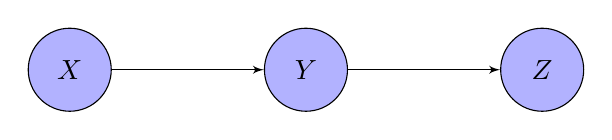
\begin{tikzpicture}[node distance=3cm,auto,>=latex',every node/.append style={align=center}]
    \node [int,  fill = white!70!blue] (a)              {$X$};
    \node [int,  fill = white!70!blue]           (c) [right of=a] {$Y$};
    \node [int,  fill = white!70!blue] (e) [right of=c] {$Z$};
    \path[->, auto=false] (a) edge node {} (c)
                          (c) edge node {} (e) ;

\end{tikzpicture}
\caption{Depiction of a SIR model where $X=S, Y=I,$ and $Z=R$.  One can only get the disease once in this model.}\label{fig::sir}
\end{figure}
An outbreak occurs if the rate of change of infectious individuals is positive, $\frac{dY}{dt} > 0$, or equivalently,
\begin{align*}
  \frac{dY}{dt} &> 0 \\
  \implies \frac{\beta X Y}{N}  - \gamma Y &> 0 ,\\
\implies  Y \left ( \beta \frac{X}{N} - \gamma \right ) & > 0\\
\implies   \frac{\beta}{\gamma} &> \frac{N}{X}.
\end{align*}
That is,  the rate of new infections is greater than the rate of recovery.  So as long as the number of susceptibles is large compared to the total population, $\frac{X}{N} \approx 1$, then an outbreak will occur if $\rr >1$,
\begin{align*}
  \rr \overset{def}{=} \frac{\beta}{\gamma} > 1.
  \end{align*}
  In order to incorporate randomness into the model, we add noise, namely,
  \begin{align}\label{eq:sir-noise}
    X_{obs}(t) &= X(t) + \epsilon_{X,t}\\
    Y_{obs}(t) &=  N - X_{obs}(t) -Y_{obs}(t)  \nonumber\\
    Z_{obs}(t) &= Z(t) - \epsilon_{Z,t}. \nonumber
  \end{align}
We are assuming the observations are generated based on the deterministic ODEs presented in Equation \ref{eq:sir} with the addition of time ($t=0, 1, \dots, T$) and compartment dependent noise $\epsilon_{X,t}$ and $\epsilon_{Z,t}$.  Since, $N$, the total population, is constant, then $Y_{obs}$ is adjusted accordingly.

In summary, when we discuss estimators for $\rr$ for the SIR model, we mean to say we are forming an estimator of $\rr$ from the given set of data in Eq. \ref{eq:sir-noise},
\begin{align*}
  \textnormal{Data} &= \left \{\left (X_{obs}(t), Y_{obs}(t), Z_{obs}(t) \right ) : t=0, 1, \dots, T\right \}, \\
  \hat{\rr} &= m(Data),
\end{align*}
where $m$ is a function of the data.

Good properties of an estimator may include being (1) being a consistent estimator
\begin{align*}
  \hat{\rr} \overset{P}{\to} 0 \textnormal{ as } T\to \infty
\end{align*}
or (2) converging to a known probability distribution,
\begin{align*}
\hat{\rr} \leadsto F.  
\end{align*}
As we are interested in the hypothesis
\begin{align*}
  H_0:\;& \rr > 1 \\
  H_A:\;& \rr \le 1
\end{align*}
Then for some $\alpha \in [0,1]$, we would like to know for some $a, b >0$
\begin{align*}
P(a \le \hat{\rr} \le b) = 1 - \alpha,  
\end{align*}
the second property is particularly desirable.  At any rate, we would like to be able to estimate $a$ and $b$ for a given $\alpha$-level.

\section{Overview of \wxxsir methods to estimate $\rr$ for the SIR model}
\label{sec:methods} 

In this section, we describe the \wxxsir methods in detail, including advantages and disadvantages of each.

\subsection{Least Squares ($\beta$, $\gamma$) (LS)}\label{least-squares-beta-gamma}
The first approach to estimate $\rr$ in the SIR model is to minimize the joint sum of squares as seen in approaches similar to \cite{malik2008} and \cite{canto2017}.  In this method, the least squares estimate of $\rr$ is formed from the data collected at each time point to estimate $\hat{\beta}$ and $\hat{\gamma}$ and uses the  subsequent plug-in estimator found in Equation \ref{eq:sirls} to estimate $\rr$.  In particular, we find

\begin{align*}
(\hat{\beta}, \hat{\gamma} )&=\arg \min_{\beta, \gamma} \sum_{t} \left [ \left (X_{obs}(t) - X(t)\right )^2 + \left ( Z_{obs}(t) - Z(t) \right )^2 \right ]
\end{align*}
Then  the estimate for $\rr$ is given by Equation \ref{eq:sirls},
\begin{align}\label{eq:sirls}
  \hat{\rr}= \frac{\hat{\beta}}{\hat{\gamma}}.
\end{align}

This method is sometimes used to estimate $\hat{\beta}$ and $\hat{\gamma}$ by using a grid search but can be done with more sophisticated minimization algorithms.  Due to the ODE format of the equations, we can only use minimization algorithms which do not rely on an explicit gradient such as Nelder-Mead simplex minimization \citep{nelder-mead1965}.

A reasonable question one may ask is why use the $L_2$-norm as opposed to $L_1$ or some other similarity score.  A possible answer is that if we were to assume Gaussian noise, then the $L_2$-norm would be equivalent to the maximum likelihood estimation.  Another answer is that $L_1$ is a continuously differentiable function and hence is easier to compute, which allows for sensitivity analysis to more easily be conducted.  Finally, LS can be done without writing down explicit assumptions on the noise within the model.  However, we cannot guarantee properties of consistency or converging to a known distribution without more explicit assumptions.

On the other hand, least squares is easy to implement in software such as base \texttt{R}'s \texttt{optim()} function, and as we see in Section \ref{sec:results}, produces comparable methods to other methods.

\subsection{Reparametrized Least Squares ($\rr$, $\gamma$) (ReLS)}\label{reparametrized-least-squares-rux5f0-gamma}

In the previous method (Section \ref{least-squares-beta-gamma}), we estimated $\beta$ and $\gamma$ and then estimated $\rr$.  However, it is possible to directly estimate $\rr$ if we reparametrize the ODEs in Equation \eqref{eq:sir} directly with \(\rr\) and \(\gamma\), using the relation $\rr = \frac{\beta}{\gamma}$,

\begin{align*}
  \left \{
  \begin{array}{cl}
    \frac{dX}{dt} &= - \rr \gamma Y \frac{X}{N}\vspace{.5em}\\
    \frac{dY}{dt} &=  \rr \gamma Y \frac{X}{N}  - \gamma Y\vspace{.5em} \\
    \frac{dZ}{dt} &=  - \gamma Y 
  \end{array}
  \right . .
  \end{align*}
We find
\begin{align*}
(\hat{\rr}, \hat{\gamma} ) &= \text{argmin}_{\rr, \gamma} \sum_{t} \left [ \left (X_{obs}(t) - X(t)\right )^2 + \left ( Z_{obs}(t) - Z(t) \right )^2 \right ]
\end{align*}
We use the $\hat{\rr}$ directly from the above estimation process, which again can be done with a grid search or another optimization process.  It may be surprising that this method leads to different results than in simply using least squares.  One reason we obtain different results may be attributed to better numerical precision as there is one fewer step to obtain an estimate for $\rr$.  However, we also see that this method results in smaller standard errors than in LS, which we discuss more in Section \ref{sec:results}.

Like LS, while we have no explicit parametric assumptions on the noise, we also are uncertain of any theoretical guarantees of our resulting estimator.  Likewise, the same difficulties in sensitivity analysis arise as in LS.



\subsection{Linear Model Approximation (LMA)}\label{linear-model-approximation-degree-10}

The SIR ODEs in Eq. \ref{eq:sir} have no known closed form solution, and so we are already using approximations using numerical integration.  In addition to this, data collected from real diseases are typically very noisy to begin with.  \cite{chang2017} discovered that an SIR model may be well approximated by a linear model.  We use this approach here to estimate $\rr$.

Specifically, we estimate two linear polynomials in \(t\) with degree \(K= 10\) to \(X_{obs}\)
and \(Y_{obs}\) using least squares to find the coefficients $\{(\hat{x}_k,
\hat{y}_k)\}_{k=1, \dots, K}$,
\begin{align*}
\hat{X}(t) &= \sum_{k=0}^K \hat{x}_k t^k\\
{\hat{Y}}(t) &= \sum_{k=0}^K \hat{y}_k t^k
\end{align*}
Then, we estimate the derivatives as
\begin{align*}
\hat{X}^\prime(t) &= \sum_{k=1}^K k \hat{x}_k t^{k-1}\\
\hat{Y}^\prime(t) &= \sum_{k=0}^K k \hat{y}_k t^{k-1}
\end{align*}
Following,  an estimator for \(\rr\) is derived from the ODEs in Equation \eqref{eq:sir},
\begin{align}
  - \frac{X^\prime}{Z^\prime}&= \rr \frac{X}{N} \nonumber\\
  \rr &=       -\frac{X^\prime}{
        Z^\prime} \cdot \frac{N}{X} \nonumber\\
  \hat{\rr} &= -\frac{\hat{X}^\prime(0)}{ \hat{Z}^\prime(0)} \cdot \frac{N}{\hat{X}(0)}. \nonumber
  \end{align}
  Here, $K=10$ is arbitrary and should be selected using some criterion such as AIC in addition with the knowledge of how many data points are available to the user.  Besides optionally deciding on the degree of polynomials to fit, this model is simple to implement and gives very comparable results to using least squares with the SIR model.  The time $t=0$ is used to best capture the initial outbreak.

  An advantage of using this estimation method is that it is simple to implement using any linear modelling software.  On the other hand, we are assuming $X(t) = \hat{X}(t)$ and so if the data truly follows a SIR model, then we will have biased estimators for $\rr$.  Using this method, we are able to check how sensitive $\rr$ is to the degree of the fitted polynomial.

\subsection{Linear Model Approximation, All Time Points (LMAT)}\label{linear-model-approximation-all-time-points-degree-10}

The above formulation (Section \ref{linear-model-approximation-degree-10}) of a linear model approximation only uses the estimate at time $t=0$ to estimate $\rr$.  We can instead, use all time points available to estimate $\rr$.  We fit a linear polynomial of \(t\) with degree \(K= 10\) model to \(X\)
and \(Z\) as above, with a slight modification in how we estimate
\(\rr\),
\begin{align*}
  \hat{\rr} &= \frac{1}{\# \text{ Obs }t} \sum_t \frac{-\hat{X}^\prime(t)}{\hat{Z}^\prime(t)} \cdot \frac{N}{X(0)} 
\end{align*}
The intuition is that $\frac{-X^\prime(t)}{Z^\prime(t)}$ is constant in $t$, but due to our approximations with the linear model, this is no longer the case.  Here, we average over the different possible values of $\rr$, estimated at different times.  An advantage to this approach is that we have a more robust estimate of $\rr$ than just using one time point.  However, the estimate will still be biased.  Like in LMAT, we can examine how sensitive $\rr$ is to the order of the polynomial $K$.


\subsection{Incidence to Prevalence Ratio (IPR)}\label{incidence-to-prevalence-ratio}
The incidence to prevalence ratio (IPR), described by \cite{Nishiura2009}, is another intuitive method to calculate $\rr$ as it incorporates some of the most basic epidemiological quantities, incidence and prevalence.

In terms of data from the SIR model, incidence $J(t) \approx -(X(t+1) - X(t))$, and the IPR$(t) = \frac{J(t)}{Y(t)}$.  This method assumes that we have some prior knowledge about $\gamma$, the transmission rate.  Thus we use as our estimate,
\begin{align*}
\hat{\rr} &= \textnormal{IPR}(t) \cdot \frac{1}{\gamma}
\end{align*}

Here we assume that the time step is small enough to approximate the incidence.  The advantage of this method is that incidence data is generally available as is prevalence data for certain diseases such as HIV \citep{hall2008}.  However, as one is required to have prior knowledge about $\gamma$, it may be easier to directly estimate $\rr$ with one of the many other methods described that does not require a prior knowledge about $\gamma$.  Again, we are using only one time point to estimate $\rr$.  This model is agnostic to assumptions on the noise, but again, it is unclear if this is an unbiased or consistent estimator of $\rr$.

\subsection{Smoothed Incidence to Prevalence Ratio (SIPR)}
We use the same method as above, IPR, but first estimate splines with 4 degrees of freedom, $\hat{X}(t)$ and $\hat{Y}(t)$, , to fit to $X_{obs}$ and $Y_{obs}$, respectively.  Then  $J(t) \approx -(\hat{X}(t+1) - \hat{X}(t))$, and the $\hat{\textnormal{IPR}}(t) = \frac{J(t)}{\hat{Y}(t)}$.  Then
\begin{align*}
\rr &= \hat{\textnormal{IPR}}(t) \cdot D
\end{align*}
The advantage of this method is that it creates a less noisy estimate than estimating IPR using only one point.  It has the same disadvantages as the regular IPR ratio in that it requires knowledge about $\gamma$.    Also, ratio estimators usually behave badly when the denominator is small.

%%%%%%%%%%%%%%%%%%%%%
\subsection{Log-Linear (LL)}
\cite{harko2014exact} were able to reduce the SIR model to one ODE.  From this, we can derive the following,
\begin{align}
  X(t) &=  X(0) e^{\frac{-\beta}{\gamma}\frac{Z(t)}{N}} \nonumber\\
  \log \frac{X(t)}{X(0)} &=  \frac{-\beta }{\gamma}\frac{Z(t)}{N} \nonumber\\
  \log \frac{X(t)}{X(0)} &=  -\rr \frac{Z(t)}{N}. \label{eq:harko_lin}
\end{align}

Thus, we can regress the left hand side in Eq. \ref{eq:harko_lin} on $Z(t)$, the number of recovered individuals, with $\rr$ as the coefficient of $Z(t)/N$ and no intercept term to obtain an estimate of $\hat{\rr}$,
\begin{align*}
  \hat{\rr} = -\frac{\sum_{t=0}^T \log \frac{ X(t)}{X(0)}}{\sum_{t=0}^T\frac{Z(t)}{N}}.
\end{align*}
This method says that for a one percent increase in number of recovered individuals, we expect the ratio of number of old susceptibles to number of new susceptibles to increase by $e^{\rr}$,
\begin{align*}
  \log \left ( X(t+1)/ X(0) \right ) - \log \left ( X(t)/X(0) \right ) &= - .01\rr\\
  \log \left ( X(t+1) \right ) - \log \left ( X(t) \right )  &=- .01\rr\\
  \log \left ( X(t) / X(t+1) \right ) &= .01\rr\\
  \frac{X(t)}{X(t+1)}  &\approx e^{\rr}.
\end{align*}

The advantages of this method are many.  One, the estimate of $\rr$ is highly interpretable.  Two, an assumption of Gaussian noise in Equation \ref{eq:harko_lin} is not as egregious as in the other methods to estimate $\rr$ because we are looking at a log transformation of the the percent of suceptibles instead of untransformed variables.  As a consequence, we may be able to make a case where we the resulting estimate of $\rr$ is unbiased and a consistent estimator.  Finally,  this method is easily implemented using any linear modelling software.  

\subsection{Markov chain estimation (MC)}
A natural approach to epidemic modeling is that of Markov chains (MC), since it is assumed an individual's next state is only dependent on its current state.  Much work has been done over the years in this specific field including asymptotic behavior, continuous time MC, confidence intervals, and more \citep{jacquez1991,gani1995,daley2001epidemic}.  We present one simple instantiation of the model, the discrete time case, which traces its origin back to the Reed-Frost model \citep{abbey1952}.

In this method, the number of susceptibles at the next step, $X(t+1)$, has a Binomial distribution based on the contacts with the current number of infectious, $Y(t)$ and the current number of susceptibles.  That is $X(t+1) \sim \text{Binomial}\left(X(t), \alpha^{Y(t)}\right)$, where $\alpha$ is the probability of avoiding infection from an infective.  One can write out the likelihood for $\alpha$ in this model, namely,
\begin{align*}
\mathcal{L}\left ( \alpha ; \textnormal{data}\right ) \propto \prod_{t=0}^{T-1}\left ( \alpha^{Y(t)} \right )^{X(t+1)} \left (1- \alpha^{Y(t)} \right )^{X(t) - X(t+1)}.
\end{align*}
Maximizing the likelihood yields an estimate for $\alpha$,
\begin{align*}
\hat{\alpha} = \arg \max_{\alpha} \mathcal{L}\left(\alpha; \textnormal{data} \right ).
  \end{align*}
 \cite{barbour2004} report that the estimated reproduction number is thus,
\begin{align}\label{eq:r0-mc}
\hat{\rr} &= \log \left ( \frac{1}{1-\hat{\alpha}}\right ).
\end{align}

This method typically allows for more than just the reproduction number to be estimated.  Through recursion, one can calculate the probability of having a given number of susceptibles and infected at each time step, and hence the entire probability distribution may be known.

The advantages of this model are its simplicity of interpretation and ability to generate a whole probability distrubtion for $(X(t), Y(t))$.  We have explicitly stated how randomness enters the model so it is up to the researcher to check whether this assumption is a good fit.  However, it is possible to simulate how sensitive $\hat{\rr}$ is to $\hat{\alpha}$.





\subsection{Sequential Bayes (SB)}\label{sec:seqbayes}

Described by \cite{bettencourt2008} and summarized in \cite{obadia2012r0}, the sequential Bayes method is a Bayesian approach to an approximation of the classic SIR model.  The approximated SIR model assumes that the incidence at $t+1$, $J(t+1)$ has a Poisson distribution, with $\gamma$ as the  average inverse of the infectious period. In order to estimate $\rr$, we must have some idea about $\gamma$,
\begin{align*}
J(t+1)  \sim \textnormal{Poisson}( J(t) \exp \left \{  \gamma (\rr-1)\right \})
\end{align*}
Then, the posterior distribution of $\rr$ given the previous days' incidences is
\begin{align*}
  P(\rr | J(0), \dots, J(t+1)) = \frac{P(J(t+1) | \rr, J(0), \dots, J(t))P(\rr| J(0), \dots, J(t))}{P(J(0), \dots, J(t+1))}.
\end{align*}
This method is sequential in that the prior distribution for $\rr$ comes from the previous day.  The initial prior for $\rr$ is assumed to be flat.  This method results in a posterior distribution from which credible intervals may be obtained.  This method assumes, initial growth in incidence to be exponential, and homogeneous mixing of populations as with any compartment model.  The advantages of this method are that of the ability to obtain an entire posterior distribution, whereas many other methods are difficult to even find an estimate of the variance.  Disadvantages include strict assumptions about the distributions and computational time required to estimate the relevant parameters. 




\section{Confidence and Credible Intervals}
\label{sec:ci}

Estimating $\rr$ is difficult and estimating $V[\rr]$, the variance and subsequently CIs, are even more so.  We describe general methods which may be applicable to estimate the variance.  In particular, we describe three methods 1) the delta method, 2) the block strap, and 3) posterior distributions.


\subsection{Delta Method}\label{delta-method}

When a method estimates \(\beta\) and \(\gamma\) instead of \(\rr\) directly, we use the delta method approximation to calculate the
variance of \(\rr\). Here, we know \(\rr = h(\beta, \gamma) = \frac{\beta}{\gamma}\). Then \(\bigtriangleup h = (\frac{1}{\gamma},  -\frac{\beta}{\gamma^2})^T\) and \(V[\rr] = \bigtriangleup h^T \Sigma_{\beta, \gamma} \bigtriangleup h\), where \(\Sigma_{\beta, \gamma}\) is covariance matrix of \(\beta\) and \(\gamma\).

This estimate assumes that the distribution of $\beta$ and $\gamma$ are asymptotically normal.  Here, we use the relationship of $\rr = \frac{\beta}{\gamma}$ in order to estimate the variance, which is specific to the SIR framework.  A disadvantage of this method is that it provides no insight on how to estimate $\Sigma_{\beta,\gamma}$.

\subsection{Block Bootstrap}

The block bootstrap is a variant of the bootstrap in which the $n$ observations are dependent on one another.  In contrast to the original bootstrap, the block bootstrap partitions consectutive observations into $k$ blocks with block-length $b$ ($n=kb$).  These are non-overlapping partitions or blocks, although there are variants for which blocks can overlap.  Following, for iteration $\ell$, one samples uniformly replacement $k$ blocks and estimates $\hat{\rr}_b$ from those $k$ blocks, repeating the sampling and estimation for a total of $L$ estimates of $\hat{\rr}$.  Then
\begin{align*}
  V\left [ \hat{\rr} \right ] &\approx V\left [\hat{\rr}_\ell \right ].
\end{align*}
More about the asympotic distributions of the blockwise-bootstrap can be found in \cite{cao1999}, along with descriptions of variants.

The assympotic properties hold when the stochastic process is $m$-dependent, that is when observations $t, t+1, \dots$ and $s, s+1, \dots$ are independent whenever $s+m < t$ and under some smoothness conditions of the statistic used to estimate $\rr$.

A choice one must make in the block bootstrap is the block size $b$.  One simple recommendation is to take $b= n^{1/3}$, which is derived from the asymptotic mean square error of the method.


\subsection{Posterior Distribution}
When one uses a Bayesian approach to estimate $\rr$, the result should be a distribution rather than an estimate.  One can simply look at the quantiles of this distribution to form a credible interval for this estimate.  Advantages of this method include having an entire distribution compared to a point estimate.  One disadvantage is that the Bayesian approach will not guarantee frequentist properties that epidemiologists may be looking for such as being able to compare diseases to one another.




%%%%%%%%%%%%%%%

\section{Methods}\label{sec:sim-res}

We compare the performance of the SIR models on simulated data from both the SIR as well as other models. In all of these simulations, we first generate data from the models under known conditions, then we add on errors with known variances to each time point. We simulate with two different types of error distributions, Gaussian and autoregressive. In the Gaussian case, we add on independently and identically distributed errors to the $X$ and $Y$ compartments with variances $\sigma_X$ and $\sigma_Y$, respectively; the sum of these errors is then subtracted from the $Z$ compartment to maintain constant population. The same process was followed for the autoregressive case, except that we generate errors from an AR(1) model with a correlation coefficient $\rho = 0.7$ added to Gaussian white noise. For each error distribution, we simulate an additional data set which adds a monotonicity adjustment to the X and Z compartments after adding on the  using the Pool Adjacent Violators Algorithm (PAVA). The sum of the populations of these compartments is then subtracted from the $Y$ compartment, again to maintain a constant population. This gives us a total of four error structures for each set of conditions: Gaussian (Norm), Gaussian monotone (Norm-M), autoregressive (AR), and autoregressive monotone (AR-M).

\subsection{SIR Data}

We first simulate 5 ``baseline'' data sets from the SIR model under the following conditions: 

\begin{center}
	
	$\beta$ = 0.06, $\gamma$ = 0.03; $\rr$ = 2
	
	Number of time steps: 365
	
	Starting X size ($X_0$): 99950
	
	Starting Y size ($Y_0$): 50
	
	Starting Z size: 0 
	
	$\sigma_X$: 100
	
	$\sigma_Y$: 5
	
	Total population: 100000.
	
\end{center}

We then generate different SIR data sets, changing the one of the conditions for simulation each time and using the baseline SIR data as our basis for comparison. The different data sets generate are shown in the following table:

\begin{table}[h]
	\centering
	\resizebox{\textwidth}{!}{
		\begin{tabular}{@{}lll@{}}
			\toprule
			\textbf{Parameter Values ($\beta, \gamma$)}        & \textbf{Starting Compartment Sizes ($X_0, Y_0$)}            & \textbf{Variance of Added Errors ($\sigma_X, \sigma_Y$ )}       \\ \midrule
			(0.06, 0.001)            & (99000, 1000)                           & (50, 2)                     \\
			(0.06, 0.04)             & (99900, 100)               & (500, 20)     \\
			(0.06, 0.06)             & (99990, 10)             & (2500, 100)           \\
			(0.06, 0.24) & (99999, 1) & (10000, 500)                                      \\ \bottomrule
		\end{tabular}
	}
	\caption{Table of data sets.}
	\label{tab:datasets}
\end{table}

\subsection{Other Models}

To test how well the SIR models perform under misspecification, we simulate data from other models. While we will not have a ``known'' $\rr$ value to compare our results to, this will allow us to see if the models give us reasonable results when the data do not come from the SIR model. We simulate data from linear and quartic models with respect to the time step, using a monotonically increasing function for the $X$ compartment and a monotonically decreasing function for the $Z$ compartment. The sum of these is subtracted from the constant total population to get the $Y$ compartment. We also generated data from a linearized version of the three compartment SIR model with the following ODEs:

\begin{eqnarray*}
	\frac{dX}{dt} &=& -\beta Y \\
	\frac{dY}{dt} &=& \beta Y - \gamma Y \\
	\frac{dZ}{dt} &=& \gamma Y.
\end{eqnarray*}

The data from the linear SIR model were simulated under the following conditions:

\begin{center}
	
	$\beta$ = 0.06, $\gamma$ = 0.05; $\rr$ = 1.2
	
	Number of time steps: 365
	
	Starting X size ($X_0$): 99950
	
	Starting Y size ($Y_0$): 50
	
	Starting Z size: 0 
	
	$\sigma_X$: 10
	
	$\sigma_Y$: 1
	
	Total population: 100000.
	
\end{center}

\section{Results}\label{sec:results}
There are numerous aspects to consider when using a method to estimate $\rr$.  Among these include values of both the infection and recovery rate $(\beta, \gamma)$, the number of data points available (time $T$), the total size of the population ($N$), the initial percent of susceptible individuals $\left (\frac{X(0)}{N}\right)$, the initial percent of infectious individuals $\left (\frac{Y(0)}{N}\right )$, and  the magnitude of the variance of both the number of susceptibles and the number of infectious ($\sigma_X, \sigma_Y$).  We examine each of these aspects individually.

\subsection{Baseline}\label{sec:res-base}


\subsection{Infection and Recovery Rate ($\beta, \gamma$)}\label{sec:res-beta-gamma}



\subsection{Number of Time Steps ($T$)}\label{sec:res-time}



\subsection{Initial Percentage of Infectious $\left (\frac{Y(0)}{N}\right)$}\label{sec:res-inf}



\subsection{Magnitude of Variance $(\sigma^2_X, \sigma^2_Y)$}\label{sec:res-var}



\subsection{Other Models}\label{sec:res-oth}



\section{Discussion}\label{sec:discussion}



\bibliographystyle{apa}%Choose a bibliograhpic style
\bibliography{Master}


\appendix

\section{Beyond the SIR Model}

\section{Fitting the SIR Model}

\subsection{SIR Least Squares}

\begin{table}[H]
	
	\caption{\label{tab:}$\rr$ Estimates and Std. Errs, SIRLS Model,
		$X_0 = 99950, Y_0 = 50$, $\sigma_X = 100, \sigma_Y = 5$,$\beta = 0.06, \gamma = 0.03$}
	\centering
	\begin{footnotesize}
		\begin{tabular}[t]{l|r|r|r|r|r|r|r|r}
			\hline
			Data Set & Norm Est & Norm SE & Norm-M Est & Norm-M SE & AR Est & AR SE & AR-M Est & AR-M SE\\
			\hline
			Baseline1 & 1.999919 & 0.0058322 & 2.000036 & 0.0044639 & 2.000020 & 0.0078308 & 2.000859 & 0.0060766\\
			\hline
			Baseline2 & 1.999971 & 0.0055923 & 2.000246 & 0.0044456 & 1.999739 & 0.0071509 & 1.999992 & 0.0073664\\
			\hline
			Baseline3 & 2.000327 & 0.0054549 & 1.999861 & 0.0048111 & 1.999165 & 0.0078453 & 2.000160 & 0.0063235\\
			\hline
			Baseline4 & 2.000520 & 0.0057238 & 1.999501 & 0.0046540 & 1.999282 & 0.0077363 & 1.999289 & 0.0065290\\
			\hline
			Baseline5 & 1.999919 & 0.0056334 & 2.000053 & 0.0045020 & 2.001443 & 0.0081239 & 2.002397 & 0.0075056\\
			\hline
		\end{tabular}
	\end{footnotesize}
\end{table}

\begin{table}[H]
	
	\caption{\label{tab:}$\rr$ Estimates and Std. Errs, SIRLS Model,
		$X_0 = 99950, Y_0 = 50$, $\sigma_X = 100, \sigma_Y = 5$, $\beta = 0.06$}
	\centering
	\begin{footnotesize}
		\begin{tabular}[t]{l|r|r|r|r|r|r|r|r}
			\hline
			Data Set & Norm Est & Norm SE & Norm-M Est & Norm-M SE & AR Est & AR SE & AR-M Est & AR-M SE\\
			\hline
			$\gamma$ = 0.001 & 59.9764682 & 0.0434705 & 59.9764682 & 0.0386733 & 60.0151171 & 0.0697888 & 59.9589126 & 0.0631448\\
			\hline
			$\gamma$ = 0.04 & 1.5000763 & 0.0126817 & 1.5001978 & 0.0090880 & 1.4989700 & 0.0182852 & 1.4993603 & 0.0165168\\
			\hline
			$\gamma$ = 0.06 & 1.0043054 & 0.4140424 & 0.9955554 & 0.1086448 & 0.9915431 & 0.6272644 & 0.9941392 & 0.1891812\\
			\hline
			$\gamma$ = 0.24 & 0.2363274 & 4.1042813 & 0.2327691 & 0.6701185 & -0.0695410 & 2.8291362 & 0.3021083 & 0.5657139\\
			\hline
		\end{tabular}
	\end{footnotesize}
\end{table}

\begin{table}[H]
	
	\caption{\label{tab:}$\rr$ Estimates and Std. Errs, SIRLS Model,
		$\sigma_X = 100, \sigma_Y = 5$, $\beta = 0.06, \gamma = 0.03$}
	\centering
	\begin{footnotesize}
		\begin{tabular}[t]{l|r|r|r|r|r|r|r|r}
			\hline
			Data Set & Norm Est & Norm SE & Norm-M Est & Norm-M SE & AR Est & AR SE & AR-M Est & AR-M SE\\
			\hline
			$X_0 = 99000, Y_0 = 1000$ & 1.999588 & 0.0049609 & 2.000284 & 0.0046294 & 2.000461 & 0.0078398 & 2.000122 & 0.0068626\\
			\hline
			$X_0 = 99900, Y_0 = 100$ & 2.022501 & 0.3064263 & 2.021865 & 0.3064148 & 2.022296 & 0.3063477 & 2.022665 & 0.3068512\\
			\hline
			$X_0 = 99990, Y_0 = 10$ & 2.116865 & 0.6626380 & 2.116551 & 0.6621184 & 2.116959 & 0.6623142 & 2.116803 & 0.6620448\\
			\hline
			$X_0 = 99999, Y_0 = 1$ & 2.468304 & 1.5370731 & 2.466776 & 1.5348981 & 2.470607 & 1.5371890 & 2.466700 & 1.5348542\\
			\hline
		\end{tabular}
	\end{footnotesize}
\end{table}

\begin{table}[H]
	\caption{\label{tab:}$\rr$ Estimates and Std. Errs, SIRLS Model,
		$X_0 = 99950, Y_0 = 50$, $\beta = 0.06, \gamma = 0.03$}
	\centering
	\begin{footnotesize}
		\begin{tabular}[t]{l|r|r|r|r|r|r|r|r}
			\hline
			Data Set & Norm Est & Norm SE & Norm-M Est & Norm-M SE & AR Est & AR SE & AR-M Est & AR-M SE\\
			\hline
			$\sigma_X = 50, \sigma_Y = 2$ & 1.993455 & 0.5784530 & 1.979966 & 0.1204126 & 2.033934 & 0.7559710 & 2.066706 & 0.3382834\\
			\hline
			$\sigma_X = 500, \sigma_Y = 20$ & 1.998088 & 0.1353803 & 1.996950 & 0.0541332 & 1.999686 & 0.1893888 & 2.002135 & 0.0927952\\
			\hline
			$\sigma_X = 2500, \sigma_Y = 100$ & 1.999755 & 0.0026502 & 1.999834 & 0.0026397 & 1.999555 & 0.0037664 & 1.999038 & 0.0036473\\
			\hline
			$\sigma_X = 10000, \sigma_Y = 500$ & 2.001870 & 0.0259428 & 1.997748 & 0.0162536 & 2.002792 & 0.0416203 & 1.997918 & 0.0257997\\
			\hline
		\end{tabular}
	\end{footnotesize}
\end{table}

\begin{table}[H]
	
	\caption{\label{tab:}$\rr$ Estimates and Std. Errs, SIRLS Model,
		$X_0 = 99950, Y_0 = 50$, $\sigma_X = 100, \sigma_Y = 5$}
	\centering
	\begin{footnotesize}
		\begin{tabular}[t]{l|r|r|r|r|r|r|r|r}
			\hline
			Data Set & Norm Est & Norm SE & Norm-M Est & Norm-M SE & AR Est & AR SE & AR-M Est & AR-M SE\\
			\hline
			1st Order & 1.051438 & 0.3782910 & 1.051420 & 0.3784628 & 1.051864 & 0.3775363 & 1.051293 & 0.3782570\\
			\hline
			4th Order & 1.769347 & 0.4226615 & 1.769136 & 0.4215768 & 1.769002 & 0.4227615 & 1.769136 & 0.4215910\\
			\hline
			Linear SIR & 1.274258 & 0.0979741 & 1.273917 & 0.0976920 & 1.273654 & 0.1000387 & 1.274007 & 0.0970809\\
			\hline
		\end{tabular}
	\end{footnotesize}
\end{table}

\begin{table}[H]
	
	\caption{\label{tab:}$\rr$ Estimates and Std. Errs, SIRLS Model,
		$\beta = 0.06, \gamma = 0.03$, $X_0 = 99950, Y_0 = 50$, $\sigma_X = 100, \sigma_Y = 5$}
	\centering
	\begin{tabular}[t]{l|r|r|r|r|r|r|r|r}
		\hline
		Data Set & Norm Est & Norm SE & Norm-M Est & Norm-M SE & AR Est & AR SE & AR-M Est & AR-M SE\\
		\hline
		T = 200 & 1.999339 & 0.0286060 & 2.000583 & 0.0204020 & 2.0006557 & 0.0357152 & 2.000722 & 0.0364659\\
		\hline
		T = 100 & 1.990754 & 0.2922125 & 1.993375 & 0.1463550 & 1.9098406 & 0.3811467 & 1.967388 & 0.2324481\\
		\hline
		T = 50 & 1.978167 & 1.1596532 & 1.856227 & 0.3825275 & 2.2720601 & 1.2900031 & 1.699976 & 0.6064311\\
		\hline
		T = 20 & 38.689552 & 106.2705193 & 5.036600 & 1.3672212 & 0.0098756 & 2.1687945 & 1.681588 & 0.4747083\\
		\hline
	\end{tabular}
\end{table}

\subsection{SIR Reparameterization}

\begin{table}[H]
	
	\caption{\label{tab:}$\rr$ Estimates and Std. Errs, SIRREPAR Model,
		$X_0 = 99950, Y_0 = 50$, $\sigma_X = 100, \sigma_Y = 5$,$\beta = 0.06, \gamma = 0.03$}
	\centering
	\begin{footnotesize}
		\begin{tabular}[t]{l|r|r|r|r|r|r|r|r}
			\hline
			Data Set & Norm Est & Norm SE & Norm-M Est & Norm-M SE & AR Est & AR SE & AR-M Est & AR-M SE\\
			\hline
			Baseline1 & 1.999708 & 0.0052113 & 2.000030 & 0.0039910 & 1.999885 & 0.0069901 & 2.001023 & 0.0054369\\
			\hline
			Baseline2 & 1.999734 & 0.0049939 & 2.000314 & 0.0039684 & 2.000046 & 0.0063859 & 1.999684 & 0.0065745\\
			\hline
			Baseline3 & 2.000604 & 0.0048757 & 2.000025 & 0.0042948 & 1.999356 & 0.0069903 & 2.000438 & 0.0056503\\
			\hline
			Baseline4 & 2.000410 & 0.0051162 & 1.999830 & 0.0041504 & 1.999885 & 0.0069068 & 1.999013 & 0.0058261\\
			\hline
			Baseline5 & 1.999830 & 0.0050288 & 1.999830 & 0.0040212 & 2.001592 & 0.0072630 & 2.002090 & 0.0067284\\
			\hline
		\end{tabular}
	\end{footnotesize}
\end{table}

\begin{table}[H]
	
	\caption{\label{tab:}$\rr$ Estimates and Std. Errs, SIRREPAR Model,
		$X_0 = 99950, Y_0 = 50$, $\sigma_X = 100, \sigma_Y = 5$, $\beta = 0.06$}
	\centering
	\begin{footnotesize}
		\begin{tabular}[t]{l|r|r|r|r|r|r|r|r}
			\hline
			Data Set & Norm Est & Norm SE & Norm-M Est & Norm-M SE & AR Est & AR SE & AR-M Est & AR-M SE\\
			\hline
			$\gamma$ = 0.001 & 59.995188 & 0.4343984 & 59.9951876 & 0.3874879 & 60.025452 & 0.6911933 & 59.9960910 & 0.6214841\\
			\hline
			$\gamma$ = 0.04 & 1.499883 & 0.0062529 & 1.5001705 & 0.0044936 & 1.499068 & 0.0090313 & 1.4993177 & 0.0081651\\
			\hline
			$\gamma$ = 0.06 & 1.004306 & 0.0501444 & 0.9955446 & 0.0117215 & 0.991558 & 0.0645788 & 0.9941511 & 0.0190525\\
			\hline
			$\gamma$ = 0.24 & 4.179525 & 2.7455569 & 3.5709590 & 0.3171284 & 5.192951 & 3.5249847 & 9.8415034 & 2.5646198\\
			\hline
		\end{tabular}
	\end{footnotesize}
\end{table}

\begin{table}[H]
	
	\caption{\label{tab:}$\rr$ Estimates and Std. Errs, SIRREPAR Model,
		$\sigma_X = 100, \sigma_Y = 5$, $\beta = 0.06, \gamma = 0.03$}
	\centering
	\begin{footnotesize}
		\begin{tabular}[t]{l|r|r|r|r|r|r|r|r}
			\hline
			Data Set & Norm Est & Norm SE & Norm-M Est & Norm-M SE & AR Est & AR SE & AR-M Est & AR-M SE\\
			\hline
			$X_0 = 99000, Y_0 = 1000$ & 1.999712 & 0.0034303 & 2.000274 & 0.0032086 & 2.000082 & 0.0053846 & 2.000014 & 0.0047509\\
			\hline
			$X_0 = 99900, Y_0 = 100$ & 2.022359 & 0.2698034 & 2.021866 & 0.2694871 & 2.022178 & 0.2696002 & 2.022530 & 0.2701860\\
			\hline
			$X_0 = 99990, Y_0 = 10$ & 2.117059 & 0.7291460 & 2.116858 & 0.7290133 & 2.116829 & 0.7288841 & 2.116534 & 0.7286543\\
			\hline
			$X_0 = 99999, Y_0 = 1$  & 2.469189 & 2.7293667 & 2.466967 & 2.7219457 & 2.470707 & 2.7245397 & 2.466483 & 2.7349248\\
			\hline
		\end{tabular}
	\end{footnotesize}
\end{table}

\begin{table}[H]
	
	\caption{\label{tab:}$\rr$ Estimates and Std. Errs, SIRREPAR Model,
		$X_0 = 99950, Y_0 = 50$, $\beta = 0.06, \gamma = 0.03$}
	\centering
	\begin{footnotesize}
		\begin{tabular}[t]{l|r|r|r|r|r|r|r|r}
			\hline
			Data Set & Norm Est & Norm SE & Norm-M Est & Norm-M SE & AR Est & AR SE & AR-M Est & AR-M SE\\
			\hline
			$\sigma_X = 50, \sigma_Y = 2$ & 1.993660 & 0.5115266 & 1.979973 & 0.1053955 & 2.033636 & 0.7059701 & 2.066476 & 0.3172823\\
			\hline
			$\sigma_X = 500, \sigma_Y = 20$ & 1.998145 & 0.1207935 & 1.997147 & 0.0481545 & 2.000194 & 0.1680126 & 2.002244 & 0.0826643\\
			\hline
			$\sigma_X = 2500, \sigma_Y = 100$ & 1.999829 & 0.0023646 & 1.999946 & 0.0023591 & 1.999885 & 0.0033514 & 1.999483 & 0.0032200\\
			\hline
			$\sigma_X = 10000, \sigma_Y = 500$ & 2.002305 & 0.0232636 & 1.997996 & 0.0144744 & 2.003065 & 0.0372826 & 1.997732 & 0.0230069\\
			\hline
		\end{tabular}
	\end{footnotesize}
\end{table}

\begin{table}[H]
	
	\caption{\label{tab:}$\rr$ Estimates and Std. Errs, SIRREPAR Model,
		$X_0 = 99950, Y_0 = 50$, $\sigma_X = 100, \sigma_Y = 5$}
	\centering
	\begin{footnotesize}
		\begin{tabular}[t]{l|r|r|r|r|r|r|r|r}
			\hline
			Data Set & Norm Est & Norm SE & Norm-M Est & Norm-M SE & AR Est & AR SE & AR-M Est & AR-M SE\\
			\hline
			1st Order & 1.051435 & 0.0259416 & 1.051397 & 0.0258690 & 1.051845 & 0.0260146 & 1.051255 & 0.0257166\\
			\hline
			4th Order & 1.769331 & 0.2796903 & 1.769079 & 0.2791191 & 1.769095 & 0.2799270 & 1.769111 & 0.2788789\\
			\hline
			Linear SIR & 1.274314 & 0.0339775 & 1.274075 & 0.0337499 & 1.274174 & 0.0345629 & 1.273799 & 0.0334192\\
			\hline
		\end{tabular}
	\end{footnotesize}
\end{table}

\begin{table}[H]
	
	\caption{\label{tab:}$\rr$ Estimates and Std. Errs, SIRREPAR Model,
		$\beta = 0.06, \gamma = 0.03$, $X_0 = 99950, Y_0 = 50$, $\sigma_X = 100, \sigma_Y = 5$}
	\centering
	\begin{tabular}[t]{l|r|r|r|r|r|r|r|r}
		\hline
		Data Set & Norm Est & Norm SE & Norm-M Est & Norm-M SE & AR Est & AR SE & AR-M Est & AR-M SE\\
		\hline
		T = 200 & 1.999428 & 0.0312814 & 2.000386 & 0.0223765 & 2.000419 & 0.0390441 & 2.000199 & 0.0402489\\
		\hline
		T = 100 & 1.991014 & 0.3940097 & 1.993501 & 0.1974773 & 1.910435 & 0.4773240 & 1.967858 & 0.3065049\\
		\hline
		T = 50 & 1.977508 & 1.8877725 & 1.856480 & 0.5810168 & 2.273215 & 2.3912219 & 1.700025 & 0.7995792\\
		\hline
		T = 20 & 22.964587 & NaN & 5.044869 & 2.1398099 & NA & NA & 1.681269 & 0.6543603\\
		\hline
	\end{tabular}
\end{table}

\subsection{SIR Linear Model Approximation}

\begin{table}[H]
	
	\caption{\label{tab:}$\rr$ Estimates and Std. Errs, SIRLMA Model,
		$X_0 = 99950, Y_0 = 50$, $\sigma_X = 100, \sigma_Y = 5$,$\beta = 0.06, \gamma = 0.03$}
	\centering
	\begin{footnotesize}
		\begin{tabular}[t]{l|r|r|r|r|r|r|r|r}
			\hline
			Data Set & Norm Est & Norm SE & Norm-M Est & Norm-M SE & AR Est & AR SE & AR-M Est & AR-M SE\\
			\hline
			Baseline 1 & 1.997416 & 0.3900006 & 2.692152 & 0.5081138 & 35.656866 & 4815.2163162 & 1.667689 & 0.1718689\\
			\hline
			Baseline 2 & 1.686364 & 0.1886132 & 1.679359 & 0.1102722 & 1.474460 & 0.1130752 & 1.534979 & 0.1496990\\
			\hline
			Baseline 3 & 1.572708 & 0.1340966 & 1.743175 & 0.1667602 & 5.345243 & 33.1125597 & 2.313202 & 0.6045124\\
			\hline
			Baseline 4 & 1.640228 & 0.1956211 & 2.046183 & 0.3959176 & 1.327043 & 0.0671306 & -3.008847 & 7.5919771\\
			\hline
			Baseline 5 & 1.590702 & 0.1685914 & 1.842150 & 0.2204031 & 1.488547 & 0.1285866 & 1.868254 & 0.2217948\\
			\hline
		\end{tabular}
	\end{footnotesize}
\end{table}

\begin{table}[H]
	
	\caption{\label{tab:}$\rr$ Estimates and Std. Errs, SIRLMA Model,
		$X_0 = 99950, Y_0 = 50$, $\sigma_X = 100, \sigma_Y = 5$, $\beta = 0.06$}
	\centering
	\begin{footnotesize}
		\begin{tabular}[t]{l|r|r|r|r|r|r|r|r}
			\hline
			Data Set & Norm Est & Norm SE & Norm-M Est & Norm-M SE & AR Est & AR SE & AR-M Est & AR-M SE\\
			\hline
			$\gamma$ = 0.001 & -117.9694856 & 101.1885824 & -55.3748542 & 10.9872264 & -19.2057935 & 5.9751126 & -183.9423408 & 277.8291528\\
			\hline
			$\gamma$ = 0.04 & 1.1087585 & 0.0863592 & -3.9728056 & 1116.1887158 & 0.9757401 & 0.0213324 & 0.7333872 & 0.1787735\\
			\hline
			$\gamma$ = 0.06 & 1.0829034 & 0.1533121 & 0.9905684 & 0.1182606 & 0.9279273 & 0.0605799 & 1.0397917 & 0.0359875\\
			\hline
			$\gamma$ = 0.24 & 0.7074613 & 0.2028765 & 0.5216530 & 0.1715628 & 0.8749860 & 0.0590753 & -49.7813412 & 5303.0302298\\
			\hline
		\end{tabular}
	\end{footnotesize}
\end{table}

\begin{table}[H]
	
	\caption{\label{tab:}$\rr$ Estimates and Std. Errs, SIRLMA Model,
		$\sigma_X = 100, \sigma_Y = 5$, $\beta = 0.06, \gamma = 0.03$}
	\centering
	\begin{footnotesize}
		\begin{tabular}[t]{l|r|r|r|r|r|r|r|r}
			\hline
			Data Set & Norm Est & Norm SE & Norm-M Est & Norm-M SE & AR Est & AR SE & AR-M Est & AR-M SE\\
			\hline
			$X_0 = 99000, Y_0 = 1000$ & -87.5945650 & 66413.128046 & -0.9999761 & 1.422640 & 4.1817846 & 3.8812899 & -10.8458320 & 288.1028935\\
			\hline
			$X_0 = 99900, Y_0 = 100$ & 0.5237886 & 1.632971 & 0.2436375 & 3.754091 & 0.7149415 & 0.9374275 & -0.3051038 & 8.8837193\\
			\hline
			$X_0 = 99990, Y_0 = 10$ & -33.0051124 & 433.594227 & -1.3382741 & 3.047220 & -0.2463189 & 1.5875310 & 0.4368556 & 0.7686276\\
			\hline
			$X_0 = 99999, Y_0 = 1$ & 10.9282204 & 19.297359 & -98.6422337 & 3113.332617 & -0.8194023 & 1.7121668 & 16.6102769 & 18.1045393\\
			\hline
		\end{tabular}
	\end{footnotesize}
\end{table}

\begin{table}[H]
	
	\caption{\label{tab:}$\rr$ Estimates and Std. Errs, SIRLMA Model,
		$X_0 = 99950, Y_0 = 50$, $\beta = 0.06, \gamma = 0.03$}
	\centering
	\begin{footnotesize}
		\begin{tabular}[t]{l|r|r|r|r|r|r|r|r}
			\hline
			Data Set & Norm Est & Norm SE & Norm-M Est & Norm-M SE & AR Est & AR SE & AR-M Est & AR-M SE\\
			\hline
			$\sigma_X = 50, \sigma_Y = 2$ & 2.0398087 & 0.2773968 & 1.626788 & 0.0864885 & 1.4643659 & 0.0750183 & 2.8515449 & 0.5540996\\
			\hline
			$\sigma_X = 500, \sigma_Y = 20$ & 1.6600538 & 1.0693161 & 1.684919 & 0.2571470 & 1.1531754 & 0.0997937 & -4.9533560 & 32.2198830\\
			\hline
			$\sigma_X = 2500, \sigma_Y = 100$ & 0.4651914 & 7.5508447 & 4.206167 & 66.2206340 & 1.0391560 & 0.0166472 & -0.1164499 & 1.9126019\\
			\hline
			$\sigma_X = 10000, \sigma_Y = 500$ & 1.0899949 & 0.1202859 & 3.976724 & 4.4279629 & 0.6981674 & 0.2429844 & 1.3944715 & 1.0825033\\
			\hline
		\end{tabular}
	\end{footnotesize}
\end{table}

\begin{table}[H]
	
	\caption{\label{tab:}$\rr$ Estimates and Std. Errs, SIRLMA Model,
		$X_0 = 99950, Y_0 = 50$, $\sigma_X = 100, \sigma_Y = 5$}
	\centering
	\begin{footnotesize}
		\begin{tabular}[t]{l|r|r|r|r|r|r|r|r}
			\hline
			Data Set & Norm Est & Norm SE & Norm-M Est & Norm-M SE & AR Est & AR SE & AR-M Est & AR-M SE\\
			\hline
			1st Order & 1.2559522 & 0.1296269 & 1.2209276 & 0.0597736 & 1.2670255 & 0.1588846 & 1.2476445 & 0.1150267\\
			\hline
			4th Order & 0.3632202 & 0.1230895 & -0.0201429 & 0.1133200 & 0.3580085 & 0.1258904 & -0.0161666 & 0.1103940\\
			\hline
			Linear SIR & 1.2191443 & 0.1093267 & 1.2067608 & 0.0480986 & 1.2146478 & 0.0627181 & 0.9503153 & 0.1066437\\
			\hline
		\end{tabular}
	\end{footnotesize}
\end{table}

\begin{table}[H]
	
	\caption{\label{tab:}$\rr$ Estimates and Std. Errs, SIRLMA Model,
		$\beta = 0.06, \gamma = 0.03$, $X_0 = 99950, Y_0 = 50$, $\sigma_X = 100, \sigma_Y = 5$}
	\centering
	\begin{tabular}[t]{l|r|r|r|r|r|r|r|r}
		\hline
		Data Set & Norm Est & Norm SE & Norm-M Est & Norm-M SE & AR Est & AR SE & AR-M Est & AR-M SE\\
		\hline
		T = 200 & 0.9496498 & 0.0825419 & 1.052892 & 0.2237478 & 1.0611334 & 0.0328849 & 0.7221436 & 0.1920598\\
		\hline
		T = 100 & 1.2374397 & 0.4953607 & 1.202445 & 0.5438859 & 0.9140701 & 0.2563191 & 1.1584230 & 0.3660429\\
		\hline
		T = 50 & 0.9720834 & 0.0507265 & 1.924122 & 1.4342312 & 3.7359315 & 59.4952531 & 0.5305768 & 1.0293919\\
		\hline
		T = 20 & 1.4418031 & 7.3163878 & 1.121779 & 1.7267097 & -5.2984368 & 65.6502768 & 0.8899288 & 0.7605429\\
		\hline
	\end{tabular}
\end{table}

\subsection{SIR Linear Model Approximation, All Time Points}

\begin{table}[H]
	
	\caption{\label{tab:}$\rr$ Estimates and Std. Errs, SIRLMAT Model,
		$X_0 = 99950, Y_0 = 50$, $\sigma_X = 100, \sigma_Y = 5$,$\beta = 0.06, \gamma = 0.03$}
	\centering
	\begin{footnotesize}
		\begin{tabular}[t]{l|r|r|r|r|r|r|r|r}
			\hline
			Data Set & Norm Est & Norm SE & Norm-M Est & Norm-M SE & AR Est & AR SE & AR-M Est & AR-M SE\\
			\hline
			Baseline 1 & 1.398016 & 0.6028170 & 1.421201 & 0.7403641 & 1.049360 & 4.8830065 & 1.401437 & 0.8194417\\
			\hline
			Baseline 2 & 1.406323 & 0.6309170 & 1.442263 & 0.9241642 & 1.369425 & 0.8681724 & 1.449109 & 0.7463529\\
			\hline
			Baseline 3 & 1.408807 & 0.6215050 & 1.358127 & 0.8493445 & 1.375713 & 1.2574743 & 1.436717 & 0.6726785\\
			\hline
			Baseline 4 & 1.387819 & 0.6177830 & 1.390251 & 0.5728970 & 1.596744 & 1.3603545 & 1.325567 & 0.6545989\\
			\hline
			Baseline 5 & 1.387599 & 0.6657501 & 1.386679 & 0.5751290 & 1.359862 & 1.0018556 & 1.538778 & 0.9068372\\
			\hline
		\end{tabular}
	\end{footnotesize}
\end{table}

\begin{table}[H]
	
	\caption{\label{tab:}$\rr$ Estimates and Std. Errs, SIRLMAT Model,
		$X_0 = 99950, Y_0 = 50$, $\sigma_X = 100, \sigma_Y = 5$, $\beta = 0.06$}
	\centering
	\begin{footnotesize}
		\begin{tabular}[t]{l|r|r|r|r|r|r|r|r}
			\hline
			Data Set & Norm Est & Norm SE & Norm-M Est & Norm-M SE & AR Est & AR SE & AR-M Est & AR-M SE\\
			\hline
			$\gamma$ = 0.001 & -2.8535930 & 193.6526107 & 7.7685771 & 103.2205552 & 76.340382 & 472.4155164 & -69.9067922 & 1603.7792325\\
			\hline
			$\gamma$ = 0.04 & 1.4369752 & 0.7498020 & 1.4719115 & 3.0719036 & 1.292978 & 0.3342698 & 1.2769691 & 0.2448445\\
			\hline
			$\gamma$ = 0.06 & 0.9847650 & 0.1423066 & 0.9945574 & 0.0160864 & 1.008112 & 0.5987452 & 1.0268632 & 0.5015724\\
			\hline
			$\gamma$ = 0.24 & 0.6746914 & 6.2471252 & 0.3871567 & 4.8817556 & 1.786500 & 15.9420420 & 0.2221191 & 5.4112205\\
			\hline
		\end{tabular}
	\end{footnotesize}
\end{table}

\begin{table}[H]
	
	\caption{\label{tab:}$\rr$ Estimates and Std. Errs, SIRLMAT Model,
		$\sigma_X = 100, \sigma_Y = 5$, $\beta = 0.06, \gamma = 0.03$}
	\centering
	\begin{footnotesize}
		\begin{tabular}[t]{l|r|r|r|r|r|r|r|r}
			\hline
			Data Set & Norm Est & Norm SE & Norm-M Est & Norm-M SE & AR Est & AR SE & AR-M Est & AR-M SE\\
			\hline
			$X_0 = 99000, Y_0 = 1000$ & 0.730610 & 4.6810416 & 0.9720592 & 0.6586069 & 3.163816 & 45.776770 & 0.9367865 & 0.8857030\\
			\hline
			$X_0 = 99900, Y_0 = 100$ & 1.236415 & 0.7388933 & 1.1744675 & 1.3957615 & 1.249219 & 0.813166 & 1.1960662 & 0.6589163\\
			\hline
			$X_0 = 99990, Y_0 = 10$ & 1.459703 & 10.9219088 & 0.8531016 & 12.5573016 & -3.846910 & 71.297410 & -0.5884883 & 39.4915091\\
			\hline
			$X_0 = 99999, Y_0 = 1$ & 1.624645 & 5.0359845 & 0.4174208 & 12.8380228 & 1.301346 & 25.850056 & 3.1746775 & 12.8142151\\
			\hline
		\end{tabular}
	\end{footnotesize}
\end{table}

\begin{table}[H]
	
	\caption{\label{tab:}$\rr$ Estimates and Std. Errs, SIRLMAT Model,
		$X_0 = 99950, Y_0 = 50$, $\beta = 0.06, \gamma = 0.03$}
	\centering
	\begin{footnotesize}
		\begin{tabular}[t]{l|r|r|r|r|r|r|r|r}
			\hline
			Data Set & Norm Est & Norm SE & Norm-M Est & Norm-M SE & AR Est & AR SE & AR-M Est & AR-M SE\\
			\hline
			$\sigma_X = 50, \sigma_Y = 2$ & 1.414863 & 0.5779651 & 1.509908 & 2.1243768 & 1.3999424 & 0.7193567 & 1.426323 & 0.6782388\\
			\hline
			$\sigma_X = 500, \sigma_Y = 20$ & 1.353711 & 1.5619894 & 1.446169 & 0.7223815 & 1.0183856 & 3.5577619 & 1.996902 & 15.7391571\\
			\hline
			$\sigma_X = 2500, \sigma_Y = 100$ & 1.287786 & 4.3947658 & 1.365338 & 3.2675366 & 1.1984800 & 1.6107382 & 0.942443 & 4.3914050\\
			\hline
			$\sigma_X = 10000, \sigma_Y = 500$ & 4.811335 & 70.6594883 & 1.500486 & 1.0046353 & 0.9241342 & 1.2799734 & 1.097322 & 3.1937985\\
			\hline
		\end{tabular}
	\end{footnotesize}
\end{table}

\begin{table}[H]
	
	\caption{\label{tab:}$\rr$ Estimates and Std. Errs, SIRLMAT Model,
		$X_0 = 99950, Y_0 = 50$, $\sigma_X = 100, \sigma_Y = 5$}
	\centering
	\begin{footnotesize}
		\begin{tabular}[t]{l|r|r|r|r|r|r|r|r}
			\hline
			Data Set & Norm Est & Norm SE & Norm-M Est & Norm-M SE & AR Est & AR SE & AR-M Est & AR-M SE\\
			\hline
			1st Order & 1.1509447 & 0.1012249 & 1.138621 & 0.1738250 & 1.147184 & 0.0681524 & 1.145189 & 0.0811484\\
			\hline
			4th Order & 0.8246203 & 6.0710436 & 1.000597 & 2.5841000 & 3.255953 & 26.3713818 & 1.385674 & 8.5430506\\
			\hline
			Linear SIR & 1.2009801 & 0.0031100 & 1.200130 & 0.0040763 & 1.203159 & 0.0148085 & 1.195875 & 0.0246927\\
			\hline
		\end{tabular}
	\end{footnotesize}
\end{table}

\begin{table}[H]
	
	\caption{\label{tab:}$\rr$ Estimates and Std. Errs, SIRLMAT Model,
		$\beta = 0.06, \gamma = 0.03$, $X_0 = 99950, Y_0 = 50$, $\sigma_X = 100, \sigma_Y = 5$}
	\centering
	\begin{tabular}[t]{l|r|r|r|r|r|r|r|r}
		\hline
		Data Set & Norm Est & Norm SE & Norm-M Est & Norm-M SE & AR Est & AR SE & AR-M Est & AR-M SE\\
		\hline
		T = 200 & 3.3442696 & 21.4895422 & 1.8327212 & 0.2855541 & 1.7170357 & 0.4970127 & 2.294206 & 6.234463\\
		\hline
		T = 100 & 1.2354159 & 3.0461522 & 2.7980661 & 3.8629146 & 0.7524086 & 2.5622573 & 3.434636 & 14.604145\\
		\hline
		T = 50 & 0.7050038 & 2.8719153 & 0.3376738 & 7.9042199 & 0.6897879 & 2.7333396 & 1.274668 & 3.840504\\
		\hline
		T = 20 & 1.0078807 & 0.1424793 & 2.7045722 & 4.8031306 & 0.5716857 & 1.3981528 & 1.449643 & 1.542269\\
		\hline
	\end{tabular}
\end{table}

\subsection{Incidence to Prevalence Ratio}

\begin{table}[H]
	
	\caption{\label{tab:}$\rr$ Estimates and Std. Errs, SIRIPR Model,
		$X_0 = 99950, Y_0 = 50$, $\sigma_X = 100, \sigma_Y = 5$,$\beta = 0.06, \gamma = 0.03$}
	\centering
	\begin{footnotesize}
		\begin{tabular}[t]{l|r|r|r|r|r|r|r|r}
			\hline
			Data Set & Norm Est & Norm SE & Norm-M Est & Norm-M SE & AR Est & AR SE & AR-M Est & AR-M SE\\
			\hline
			Baseline 1 & 2.592974 & 9.040841 & 0.7282379 & 1.286539 & 2.183371 & 7.397726 & 0.7645942 & 1.862201\\
			\hline
			Baseline 2 & 2.210182 & 6.179671 & 0.7485576 & 1.504683 & 1.712691 & 5.071385 & 0.7513498 & 1.560614\\
			\hline
			Baseline 3 & 2.306256 & 6.684895 & 0.7206976 & 1.230857 & 1.718776 & 4.593769 & 0.8374593 & 2.542060\\
			\hline
			Baseline 4 & 2.547665 & 9.843667 & 0.8478792 & 2.387153 & 1.817153 & 5.771054 & 0.8604847 & 2.307269\\
			\hline
			Baseline 5 & 2.224111 & 6.227286 & 0.8080670 & 2.043471 & 1.859343 & 4.996316 & 0.7686838 & 2.308889\\
			\hline
		\end{tabular}
	\end{footnotesize}
\end{table}

\begin{table}[H]
	
	\caption{\label{tab:}$\rr$ Estimates and Std. Errs, SIRIPR Model,
		$X_0 = 99950, Y_0 = 50$, $\sigma_X = 100, \sigma_Y = 5$, $\beta = 0.06$}
	\centering
	\begin{footnotesize}
		\begin{tabular}[t]{l|r|r|r|r|r|r|r|r}
			\hline
			Data Set & Norm Est & Norm SE & Norm-M Est & Norm-M SE & AR Est & AR SE & AR-M Est & AR-M SE\\
			\hline
			$\gamma$ = 0.001 & 54.146506 & 200.2595 & 24.408675 & 66.166769 & 58.723744 & 219.989055 & 28.5230747 & 120.928788\\
			\hline
			$\gamma$ = 0.04 & 4.771508 & 12.8533 & 1.387753 & 2.630779 & 3.613754 & 8.536531 & 1.3965600 & 2.840997\\
			\hline
			$\gamma$ = 0.06 & 19.828076 & 29.1272 & 1.121667 & 4.400499 & 15.651052 & 23.539321 & 1.1251847 & 4.900022\\
			\hline
			$\gamma$ = 0.24 & 181.015802 & 742.1088 & 6.672760 & 89.936233 & 148.308767 & 740.018239 & 0.8145271 & 11.870908\\
			\hline
		\end{tabular}
	\end{footnotesize}
\end{table}

\begin{table}[H]
	
	\caption{\label{tab:}$\rr$ Estimates and Std. Errs, SIRIPR Model,
		$\sigma_X = 100, \sigma_Y = 5$, $\beta = 0.06, \gamma = 0.03$}
	\centering
	\begin{footnotesize}
		\begin{tabular}[t]{l|r|r|r|r|r|r|r|r}
			\hline
			Data Set & Norm Est & Norm SE & Norm-M Est & Norm-M SE & AR Est & AR SE & AR-M Est & AR-M SE\\
			\hline
			$X_0 = 99000, Y_0 = 1000$ & 1.285071 & 1.440980 & 0.9866029 & 1.057043 & 1.193594 & 1.195820 & 0.9960353 & 0.9987062\\
			\hline
			$X_0 = 99900, Y_0 = 100$ & 2.943264 & 7.736638 & 1.4707234 & 3.367245 & 2.230244 & 4.859448 & 1.4236604 & 2.8121697\\
			\hline
			$X_0 = 99990, Y_0 = 10$ & 18.663014 & 67.156845 & 1.8455795 & 5.401173 & 16.739763 & 71.982690 & 1.6417916 & 4.4145381\\
			\hline
			$X_0 = 99999, Y_0 = 1$ & 774.274659 & 7491.005080 & 3.6060918 & 26.540940 & 229.184142 & 1199.155653 & 2.5082330 & 12.8639109\\
			\hline
		\end{tabular}
	\end{footnotesize}
\end{table}

\begin{table}[H]
	
	\caption{\label{tab:}$\rr$ Estimates and Std. Errs, SIRIPR Model,
		$X_0 = 99950, Y_0 = 50$, $\beta = 0.06, \gamma = 0.03$}
	\centering
	\begin{footnotesize}
		\begin{tabular}[t]{l|r|r|r|r|r|r|r|r}
			\hline
			Data Set & Norm Est & Norm SE & Norm-M Est & Norm-M SE & AR Est & AR SE & AR-M Est & AR-M SE\\
			\hline
			$\sigma_X = 50, \sigma_Y = 2$ & 2.760752 & 8.131869 & 1.450899 & 2.052241 & 2.19804 & 5.456857 & 1.446505 & 2.182072\\
			\hline
			$\sigma_X = 50, \sigma_Y = 25$ & 17.377923 & 71.374848 & 1.889790 & 8.177704 & 12.91733 & 41.063025 & 2.373601 & 20.983311\\
			\hline
			$\sigma_X = 2500, \sigma_Y = 100$ & 81.490167 & 348.735085 & 2.267162 & 17.058029 & 195.37080 & 1451.040149 & 2.924092 & 18.434409\\
			\hline
			$\sigma_X = 10000, \sigma_Y = 500$ & 239.809101 & 1298.136206 & 4.500556 & 59.404233 & 92.10901 & 272.487471 & 3.535111 & 22.583706\\
			\hline
		\end{tabular}
	\end{footnotesize}
\end{table}

\begin{table}[H]
	
	\caption{\label{tab:}$\rr$ Estimates and Std. Errs, SIRIPR Model,
		$X_0 = 99950, Y_0 = 50$, $\sigma_X = 100, \sigma_Y = 5$}
	\centering
	\begin{footnotesize}
		\begin{tabular}[t]{l|r|r|r|r|r|r|r|r}
			\hline
			Data Set & Norm Est & Norm SE & Norm-M Est & Norm-M SE & AR Est & AR SE & AR-M Est & AR-M SE\\
			\hline
			1st Order & 2.699973 & 9.131131 & 2.297208 & 7.14196 & 4.334767 & 41.325146 & 4.194341 & 36.201142\\
			\hline
			4th Order & 6.260963 & 20.337163 & 5.924029 & 17.81136 & 6.268500 & 20.536192 & 5.892582 & 17.341763\\
			\hline
			Linear SIR & 1.516803 & 1.554241 & 1.208578 & 1.12544 & 1.379871 & 1.311406 & 1.208521 & 1.003065\\
			\hline
		\end{tabular}
	\end{footnotesize}
\end{table}

\begin{table}[H]
	
	\caption{\label{tab:}$\rr$ Estimates and Std. Errs, SIRIPR Model,
		$\beta = 0.06, \gamma = 0.03$, $X_0 = 99950, Y_0 = 50$, $\sigma_X = 100, \sigma_Y = 5$}
	\centering
	\begin{tabular}[t]{l|r|r|r|r|r|r|r|r}
		\hline
		Data Set & Norm Est & Norm SE & Norm-M Est & Norm-M SE & AR Est & AR SE & AR-M Est & AR-M SE\\
		\hline
		T = 200 & 7.345813 & 16.12889 & 2.048281 & 3.959862 & 5.553952 & 13.33904 & 2.052063 & 4.119090\\
		\hline
		T = 100 & 12.683604 & 21.50385 & 2.278429 & 5.329775 & 9.221913 & 18.11852 & 2.245441 & 5.708995\\
		\hline
		T = 50 & 19.220693 & 27.75807 & 2.470106 & 6.581896 & 14.757521 & 24.04262 & 2.616444 & 7.417433\\
		\hline
		T = 20 & 25.731306 & 35.29261 & 1.415537 & 4.565460 & 20.489247 & 33.72596 & 3.885644 & 8.289876\\
		\hline
	\end{tabular}
\end{table}

\subsection{Smoothed Incidence to Prevalence Ratio}

\begin{table}[H]
	
	\caption{\label{tab:}$\rr$ Estimates and Std. Errs, SIRSIPR Model,
		$X_0 = 99950, Y_0 = 50$, $\sigma_X = 100, \sigma_Y = 5$,$\beta = 0.06, \gamma = 0.03$}
	\centering
	\begin{footnotesize}
		\begin{tabular}[t]{l|r|r|r|r|r|r|r|r}
			\hline
			Data Set & Norm Est & Norm SE & Norm-M Est & Norm-M SE & AR Est & AR SE & AR-M Est & AR-M SE\\
			\hline
			Baseline 1 & 0.9251762 & $<$ 1e-07 & 0.8588266 & $<$ 1e-07 & 0.8386350 & $<$ 1e-07 & 0.7745969 & $<$ 1e-07\\
			\hline
			Baseline 2 & 0.9435412 & $<$ 1e-07 & 0.9081552 & $<$ 1e-07 & 0.8792348 & $<$ 1e-07 & 0.6976176 & $<$ 1e-07\\
			\hline
			Baseline 3 & 0.9694855 & $<$ 1e-07 & 0.9183543 & $<$ 1e-07 & 1.0065755 & $<$ 1e-07 & 0.7129407 & $<$ 1e-07\\
			\hline
			Baseline 4 & 0.9811143 & $<$ 1e-07 & 0.8743186 & $<$ 1e-07 & 0.8665770 & $<$ 1e-07 & 0.9207903 & $<$ 1e-07\\
			\hline
			Baseline 5 & 0.9276948 & $<$ 1e-07 & 0.9107829 & $<$ 1e-07 & 1.1514790 & $<$ 1e-07 & 0.7694052 & $<$ 1e-07\\
			\hline
		\end{tabular}
	\end{footnotesize}
\end{table}

\begin{table}[H]
	
	\caption{\label{tab:}$\rr$ Estimates and Std. Errs, SIRSIPR Model,
		$X_0 = 99950, Y_0 = 50$, $\sigma_X = 100, \sigma_Y = 5$, $\beta = 0.06$}
	\centering
	\begin{footnotesize}
		\begin{tabular}[t]{l|r|r|r|r|r|r|r|r}
			\hline
			Data Set & Norm Est & Norm SE & Norm-M Est & Norm-M SE & AR Est & AR SE & AR-M Est & AR-M SE\\
			\hline
			$\gamma$ = 0.001 & 3.9645187 & $<$ 1e-07 & 3.8285414 & $<$ 1e-07 & 3.9055582 & 0.000000 & 3.7112781 & $<$ 1e-07 \\
			\hline
			$\gamma$ = 0.04 & 1.7451025 & $<$ 1e-07 & 2.8785564 & $<$ 1e-07 & 68.7390000 & 0.000000 & 1.2465750 & $<$ 1e-07 \\
			\hline
			$\gamma$ = 0.06 & 0.9919790 & 0.0559052 & 0.9925620 & 0.0297783 & 0.8718278 & 0.087266 & 1.0294124 & 0.0510585\\
			\hline
			$\gamma$ = 0.24 & -0.2484284 & 0.1159769 & -0.0317365 & 0.0335514 & -2.8642901 & 0.000000 & 0.7365437 & 0.0675331\\
			\hline
		\end{tabular}
	\end{footnotesize}
\end{table}

\begin{table}[H]
	
	\caption{\label{tab:}$\rr$ Estimates and Std. Errs, SIRSIPR Model,
		$\sigma_X = 100, \sigma_Y = 5$, $\beta = 0.06, \gamma = 0.03$}
	\centering
	\begin{footnotesize}
		\begin{tabular}[t]{l|r|r|r|r|r|r|r|r}
			\hline
			Data Set & Norm Est & Norm SE & Norm-M Est & Norm-M SE & AR Est & AR SE & AR-M Est & AR-M SE\\
			\hline
			$X_0 = 99000, Y_0 = 1000$ & 2.0870176 & 57.9229822 & 2.016608 & 57.8153675 & 2.285424 & 57.4382982 & 1.922192 & 57.0457534\\
			\hline
			$X_0 = 99900, Y_0 = 100$ & -0.8808153 & $<$ 1e-07 & -1.150393 & $<$ 1e-07 & -6.563660 & $<$ 1e-07 & -1.777316 & $<$ 1e-07 \\
			\hline
			$X_0 = 99990, Y_0 = 10$ & 1.3451986 & 0.3236824 & 1.354925 & 0.3158698 & 1.381198 & 0.3093223 & 1.345069 & 0.3258082\\
			\hline
			$X_0 = 99999, Y_0 = 1$ & 2.4390757 & $<$ 1e-07 & 5.411582 & $<$ 1e-07 & 1.204689 & $<$ 1e-07 & 1.035624 & $<$ 1e-07 \\
			\hline
		\end{tabular}
	\end{footnotesize}
\end{table}

\begin{table}[H]
	
	\caption{\label{tab:}$\rr$ Estimates and Std. Errs, SIRSIPR Model,
		$X_0 = 99950, Y_0 = 50$, $\beta = 0.06, \gamma = 0.03$}
	\centering
	\begin{footnotesize}
		\begin{tabular}[t]{l|r|r|r|r|r|r|r|r}
			\hline
			Data Set & Norm Est & Norm SE & Norm-M Est & Norm-M SE & AR Est & AR SE & AR-M Est & AR-M SE\\
			\hline
			$\sigma_X = 50, \sigma_Y = 2$ & 1.836824 & $<$ 1e-07 & 1.7778150 & $<$ 1e-07 & 1.7603970 & $<$ 1e-07 & 1.842289 & $<$ 1e-07\\
			\hline
			$\sigma_X = 500, \sigma_Y = 25$ & 3.193066 & $<$ 1e-07 & 1.3211468 & $<$ 1e-07 & 1.3509726 & $<$ 1e-07 & 1.334458 & $<$ 1e-07\\
			\hline
			$\sigma_X = 2500, \sigma_Y = 100$ & 1.060609 & $<$ 1e-07 & 1.2345884 & $<$ 1e-07 & 1.7027546 & $<$ 1e-07 & 2.596160 & $<$ 1e-07\\
			\hline
			$\sigma_X = 10000, \sigma_Y = 500$ & -2.535946 & $<$ 1e-07 & 0.7094139 & $<$ 1e-07 & 0.8911487 & $<$ 1e-07 & -1.103940 & $<$ 1e-07\\
			\hline
		\end{tabular}
	\end{footnotesize}
\end{table}

\begin{table}[H]
	
	\caption{\label{tab:}$\rr$ Estimates and Std. Errs, SIRSIPR Model,
		$X_0 = 99950, Y_0 = 50$, $\sigma_X = 100, \sigma_Y = 5$}
	\centering
	\begin{footnotesize}
		\begin{tabular}[t]{l|r|r|r|r|r|r|r|r}
			\hline
			Data Set & Norm Est & Norm SE & Norm-M Est & Norm-M SE & AR Est & AR SE & AR-M Est & AR-M SE\\
			\hline
			1st Order & 58.836635 & $<$ 1e-07 & 27.429685 & $<$ 1e-07 & 1.498805 & $<$ 1e-07 & -14.135196 & $<$ 1e-07 \\
			\hline
			4th Order & 2.848624 & $<$ 1e-07 & 15.083621 & $<$ 1e-07 & 2.766152 & $<$ 1e-07 & 14.972580 & $<$ 1e-07 \\
			\hline
			Linear SIR & 1.294079 & 0.2151131 & 1.294364 & 0.2158095 & 1.296731 & 0.2215603 & 1.304489 & 0.2299876\\
			\hline
		\end{tabular}
	\end{footnotesize}
\end{table}

\begin{table}[H]
	
	\caption{\label{tab:}$\rr$ Estimates and Std. Errs, SIRSIPR Model,
		$\beta = 0.06, \gamma = 0.03$, $X_0 = 99950, Y_0 = 50$, $\sigma_X = 100, \sigma_Y = 5$}
	\centering
	\begin{tabular}[t]{l|r|r|r|r|r|r|r|r}
		\hline
		Data Set & Norm Est & Norm SE & Norm-M Est & Norm-M SE & AR Est & AR SE & AR-M Est & AR-M SE\\
		\hline
		T = 200 & -2.119890 & 0.000000 & 2.6624046 & 0.0000000 & 3.3187716 & 0.0000000 & 2.363125 & 32.2727752\\
		\hline
		T = 100 & 2.341119 & 1.168462 & 2.2020092 & 0.5643447 & 2.0919450 & 1.0699219 & 1.963112 & 0.3489431\\
		\hline
		T = 50 & 2.190565 & 2.238582 & 1.9477092 & 0.4198946 & 1.8701913 & 0.7519526 & 2.279451 & 0.6584392\\
		\hline
		T = 20 & 4.177245 & 7.320297 & 0.9702882 & 0.8673670 & 0.3570221 & 7.6611297 & 3.984916 & 2.1350792\\
		\hline
	\end{tabular}
\end{table}

\subsection{SIR Log Linear}

\begin{table}[H]
	
	\caption{\label{tab:}$\rr$ Estimates and Std. Errs, LOGLINEAR Model,
		$X_0 = 99950, Y_0 = 50$, $\sigma_X = 100, \sigma_Y = 5$,$\beta = 0.06, \gamma = 0.03$}
	\centering
	\begin{footnotesize}
		\begin{tabular}[t]{l|r|r|r|r|r|r|r|r}
			\hline
			Data Set & Norm Est & Norm SE & Norm-M Est & Norm-M SE & AR Est & AR SE & AR-M Est & AR-M SE\\
			\hline
			Baseline1 & 1.999840 & 0.0002227 & 1.999761 & 0.0001427 & 1.999820 & 0.0003227 & 2.000443 & 0.0001910\\
			\hline
			Baseline2 & 1.999807 & 0.0002198 & 2.000303 & 0.0001342 & 2.000000 & 0.0002885 & 1.999556 & 0.0002342\\
			\hline
			Baseline3 & 2.000386 & 0.0002191 & 2.000042 & 0.0001598 & 1.998138 & 0.0003215 & 1.999213 & 0.0002316\\
			\hline
			Baseline4 & 2.000039 & 0.0002252 & 1.999710 & 0.0001506 & 1.999217 & 0.0002895 & 1.999525 & 0.0002144\\
			\hline
			Baseline5 & 2.000148 & 0.0002194 & 1.999993 & 0.0001479 & 2.001889 & 0.0003495 & 2.001873 & 0.0002438\\
			\hline
		\end{tabular}
	\end{footnotesize}
\end{table}

\begin{table}[H]
	
	\caption{\label{tab:}$\rr$ Estimates and Std. Errs, LOGLINEAR Model,
		$X_0 = 99950, Y_0 = 50$, $\sigma_X = 100, \sigma_Y = 5$, $\beta = 0.06$}
	\centering
	\begin{footnotesize}
		\begin{tabular}[t]{l|r|r|r|r|r|r|r|r}
			\hline
			Data Set & Norm Est & Norm SE & Norm-M Est & Norm-M SE & AR Est & AR SE & AR-M Est & AR-M SE\\
			\hline
			$\gamma$ = 0.001 & 46.3209595 & 0.7797216 & 59.8300371 & 0.1079267 & 41.897714 & 0.9767785 & 70.7075929 & 0.9517239\\
			\hline
			$\gamma$ = 0.04 & 1.5002728 & 0.0001905 & 1.5000436 & 0.0000928 & 1.499516 & 0.0002653 & 1.5000445 & 0.0001481\\
			\hline
			$\gamma$ = 0.06 & 0.9989449 & 0.0007428 & 0.9994831 & 0.0003320 & 1.000275 & 0.0010605 & 1.0008545 & 0.0004910\\
			\hline
			$\gamma$ = 0.24 & 0.9912397 & 0.0030505 & 0.8623034 & 0.0087543 & 1.001367 & 0.0025488 & 0.9198973 & 0.0052616\\
			\hline
		\end{tabular}
	\end{footnotesize}
\end{table}

\begin{table}[H]
	
	\caption{\label{tab:}$\rr$ Estimates and Std. Errs, LOGLINEAR Model,
		$\sigma_X = 100, \sigma_Y = 5$, $\beta = 0.06, \gamma = 0.03$}
	\centering
	\begin{footnotesize}
		\begin{tabular}[t]{l|r|r|r|r|r|r|r|r}
			\hline
			Data Set & Norm Est & Norm SE & Norm-M Est & Norm-M SE & AR Est & AR SE & AR-M Est & AR-M SE\\
			\hline
			$X_0 = 99000, Y_0 = 1000$ & 1.999515 & 0.0002828 & 2.000144 & 0.0001594 & 1.999753 & 0.0004197 & 2.000586 & 0.0003024\\
			\hline
			$X_0 = 99900, Y_0 = 100$ & 2.000011 & 0.0002315 & 1.999732 & 0.0001526 & 2.000473 & 0.0002776 & 2.000640 & 0.0002656\\
			\hline
			$X_0 = 99990, Y_0 = 10$ & 1.999886 & 0.0002517 & 1.999599 & 0.0001361 & 2.000608 & 0.0003289 & 1.999049 & 0.0002664\\
			\hline
			$X_0 = 99999, Y_0 = 1$ & 1.999690 & 0.0007731 & 2.000503 & 0.0003700 & 2.002716 & 0.0010572 & 1.999919 & 0.0005663\\
			\hline
		\end{tabular}
	\end{footnotesize}
\end{table}

\begin{table}[H]
	
	\caption{\label{tab:}$\rr$ Estimates and Std. Errs, LOGLINEAR Model,
		$X_0 = 99950, Y_0 = 50$, $\beta = 0.06, \gamma = 0.03$}
	\centering
	\begin{footnotesize}
		\begin{tabular}[t]{l|r|r|r|r|r|r|r|r}
			\hline
			Data Set & Norm Est & Norm SE & Norm-M Est & Norm-M SE & AR Est & AR SE & AR-M Est & AR-M SE\\
			\hline
			$\sigma_X = 50, \sigma_Y = 2$ & 2.059934 & 0.0246402 & 1.995133 & 0.0038894 & 2.209575 & 0.0439100 & 2.545819 & 0.0568537\\
			\hline
			$\sigma\_X = 500, \sigma_Y = 20$ & 2.001882 & 0.0054085 & 1.995742 & 0.0015419 & 2.038646 & 0.0081562 & 2.015675 & 0.0031322\\
			\hline
			$\sigma\_X = 2500, \sigma_Y = 100$ & 1.999891 & 0.0001037 & 2.000036 & 0.0000930 & 1.999143 & 0.0001394 & 1.999749 & 0.0001328\\
			\hline
			$\sigma\_X = 10000, \sigma_Y = 500$ & 2.003402 & 0.0010320 & 1.998765 & 0.0003682 & 2.003763 & 0.0015505 & 1.999829 & 0.0008545\\
			\hline
		\end{tabular}
	\end{footnotesize}
\end{table}

\begin{table}[H]
	
	\caption{\label{tab:}$\rr$ Estimates and Std. Errs, LOGLINEAR Model,
		$X_0 = 99950, Y_0 = 50$, $\sigma_X = 100, \sigma_Y = 5$}
	\centering
	\begin{footnotesize}
		\begin{tabular}[t]{l|r|r|r|r|r|r|r|r}
			\hline
			Data Set & Norm Est & Norm SE & Norm-M Est & Norm-M SE & AR Est & AR SE & AR-M Est & AR-M SE\\
			\hline
			1st Order & 1.188050 & 0.0006341 & 1.187976 & 0.0006389 & 1.187553 & 0.0006273 & 1.187848 & 0.0006497\\
			\hline
			4th Order & 1.955180 & 0.0164608 & 1.955313 & 0.0164212 & 1.955130 & 0.0164623 & 1.955302 & 0.0164165\\
			\hline
			Linear SIR & 1.258587 & 0.0010079 & 1.258670 & 0.0010069 & 1.258920 & 0.0009938 & 1.258462 & 0.0010199\\
			\hline
		\end{tabular}
	\end{footnotesize}
\end{table}

\begin{table}[H]
	
	\caption{\label{tab:}$\rr$ Estimates and Std. Errs, LOGLINEAR Model,
		$\beta = 0.06, \gamma = 0.03$, $X_0 = 99950, Y_0 = 50$, $\sigma_X = 100, \sigma_Y = 5$}
	\centering
	\begin{tabular}[t]{l|r|r|r|r|r|r|r|r}
		\hline
		Data Set & Norm Est & Norm SE & Norm-M Est & Norm-M SE & AR Est & AR SE & AR-M Est & AR-M SE\\
		\hline
		T = 200 & 2.001415 & 0.0017620 & 2.000649 & 0.0009166 & 2.0053322 & 0.0023026 & 1.992983 & 0.0019266\\
		\hline
		T = 100 & 1.869996 & 0.0322729 & 1.992759 & 0.0104984 & 1.7390224 & 0.0357848 & 2.052393 & 0.0208558\\
		\hline
		T = 50 & 1.193299 & 0.0560189 & 1.741553 & 0.0454525 & 1.2098418 & 0.0420061 & 1.690908 & 0.0406272\\
		\hline
		T = 20 & 1.042976 & 0.0276261 & 1.747193 & 0.3635417 & 0.9170623 & 0.0337569 & 1.432791 & 0.0397426\\
		\hline
	\end{tabular}
\end{table}

\subsection{SIR Markov Chain}

\begin{table}[H]
	
	\caption{\label{tab:}$\rr$ Estimates and Std. Errs, SIRMC Model,
		$X_0 = 99950, Y_0 = 50$, $\sigma_X = 100, \sigma_Y = 5$,$\beta = 0.06, \gamma = 0.03$}
	\centering
	\begin{footnotesize}
		\begin{tabular}[t]{l|r|r|r|r|r|r|r|r}
			\hline
			Data Set & Norm Est & Norm SE & Norm-M Est & Norm-M SE & AR Est & AR SE & AR-M Est & AR-M SE\\
			\hline
			Baseline1 & 0.9485555 & $<$ 1e-07 & 0.9485555 & $<$ 1e-07 & 0.9485555 & $<$ 1e-07 & 0.9485555 & $<$ 1e-07\\
			\hline
			Baseline2 & 0.9485555 & $<$ 1e-07 & 0.9485555 & $<$ 1e-07 & 0.9485555 & $<$ 1e-07 & 0.9485555 & $<$ 1e-07\\
			\hline
			Baseline3 & 0.9485555 & $<$ 1e-07 & 0.9485555 & $<$ 1e-07 & 0.9485555 & $<$ 1e-07 & 0.9485555 & $<$ 1e-07\\
			\hline
			Baseline4 & 0.9485555 & $<$ 1e-07 & 0.9485555 & $<$ 1e-07 & 0.9485555 & $<$ 1e-07 & 0.9485555 & $<$ 1e-07\\
			\hline
			Baseline5 & 0.9485555 & $<$ 1e-07 & 0.9485555 & $<$ 1e-07 & 0.9485555 & $<$ 1e-07 & 0.9485555 & $<$ 1e-07\\
			\hline
		\end{tabular}
	\end{footnotesize}
\end{table}

\begin{table}[H]
	
	\caption{\label{tab:}$\rr$ Estimates and Std. Errs, SIRMC Model,
		$X_0 = 99950, Y_0 = 50$, $\sigma_X = 100, \sigma_Y = 5$, $\beta = 0.06$}
	\centering
	\begin{footnotesize}
		\begin{tabular}[t]{l|r|r|r|r|r|r|r|r}
			\hline
			Data Set & Norm Est & Norm SE & Norm-M Est & Norm-M SE & AR Est & AR SE & AR-M Est & AR-M SE\\
			\hline
			$\gamma$ = 0.001 & 0.9485554 & 1.0e-07 & 0.9485555 & $<$ 1e-07 & 0.9485555 & $<$ 1e-07 & 0.9485555 & 0e+00\\
			\hline
			$\gamma$ = 0.04 & 0.9485555 & $<$ 1e-07 & 0.9485555 & $<$ 1e-07 & 0.9485555 & $<$ 1e-07 & 0.9485555 & 0e+00\\
			\hline
			$\gamma$ = 0.06 & 0.9485555 & 2.0e-07 & 0.9485555 & $<$ 1e-07 & 0.9485555 & 2.00e-07 & 0.9485555 & 0e+00\\
			\hline
			$\gamma$ = 0.24 & 0.9485812 & 1.5e-05 & 0.9485605 & 1.4e-06 & 0.9486128 & 1.26e-05 & 0.9485558 & 2e-07\\
			\hline
		\end{tabular}
	\end{footnotesize}
\end{table}

\begin{table}[H]
	
	\caption{\label{tab:}$\rr$ Estimates and Std. Errs, SIRMC Model,
		$\sigma_X = 100, \sigma_Y = 5$, $\beta = 0.06, \gamma = 0.03$}
	\centering
	\begin{footnotesize}
		\begin{tabular}[t]{l|r|r|r|r|r|r|r|r}
			\hline
			Data Set & Norm Est & Norm SE & Norm-M Est & Norm-M SE & AR Est & AR SE & AR-M Est & AR-M SE\\
			\hline
			$X_0 = 99000, Y_0 = 1000$ & 0.9485555 & $<$ 1e-07 & 0.9485555 & $<$ 1e-07 & 0.9485555 & $<$ 1e-07 & 0.9485555 & $<$ 1e-07\\
			\hline
			$X_0 = 99900, Y_0 = 100$ & 0.9485555 & $<$ 1e-07 & 0.9485555 & $<$ 1e-07 & 0.9485555 & $<$ 1e-07 & 0.9485555 & $<$ 1e-07\\
			\hline
			$X_0 = 99990, Y_0 = 10$ & 0.9485552 & 2.00e-07 & 0.9485555 & $<$ 1e-07 & 0.9485558 & 2.0e-07 & 0.9485555 & $<$ 1e-07\\
			\hline
			$X_0 = 99999, Y_0 = 1$ & 0.9486030 & 1.56e-05 & 0.9485557 & $<$ 1e-07 & 0.9485701 & 2.6e-06 & 0.9485555 & $<$ 1e-07\\
			\hline
		\end{tabular}
	\end{footnotesize}
\end{table}

\begin{table}[H]
	
	\caption{\label{tab:}$\rr$ Estimates and Std. Errs, SIRMC Model,
		$X_0 = 99950, Y_0 = 50$, $\beta = 0.06, \gamma = 0.03$}
	\centering
	\begin{footnotesize}
		\begin{tabular}[t]{l|r|r|r|r|r|r|r|r}
			\hline
			Data Set & Norm Est & Norm SE & Norm-M Est & Norm-M SE & AR Est & AR SE & AR-M Est & AR-M SE\\
			\hline
			$\sigma_X = 50, \sigma_Y = 2$ & 0.9485506 & 3.8e-06 & 0.9485556 & 2e-07 & 0.9485428 & 2.6e-06 & 0.9485538 & 8e-07\\
			\hline
			$\sigma\_X = 500, \sigma_Y = 20$ & 0.9485562 & 1.0e-06 & 0.9485554 & 1e-07 & 0.9485640 & 3.6e-06 & 0.9485554 & 1e-07\\
			\hline
			$\sigma\_X = 2500, \sigma_Y = 100$ & 0.9485555 & $<$ 1e-07 & 0.9485555 & $<$ 1e-07 & 0.9485555 & $<$ 1e-07 & 0.9485555 & 0e+00\\
			\hline
			$\sigma\_X = 10000, \sigma_Y = 500$ & 0.9485554 & 2.0e-07 & 0.9485555 & $<$ 1e-07 & 0.9485554 & 1.0e-07 & 0.9485555 & 1e-07\\
			\hline
		\end{tabular}
	\end{footnotesize}
\end{table}

\begin{table}[H]
	
	\caption{\label{tab:}$\rr$ Estimates and Std. Errs, SIRMC Model,
		$X_0 = 99950, Y_0 = 50$, $\sigma_X = 100, \sigma_Y = 5$}
	\centering
	\begin{footnotesize}
		\begin{tabular}[t]{l|r|r|r|r|r|r|r|r}
			\hline
			Data Set & Norm Est & Norm SE & Norm-M Est & Norm-M SE & AR Est & AR SE & AR-M Est & AR-M SE\\
			\hline
			1st Order & 0.9485551 & 1e-07 & 0.9485540 & 4e-07 & 0.9485555 & 2e-07 & 0.9485553 & 2.0e-07\\
			\hline
			4th Order & 0.9485545 & 6e-07 & 0.9485533 & 1e-06 & 0.9485535 & 9e-07 & 0.9485527 & 1.2e-06\\
			\hline
			Linear SIR & 0.9485555 & $<$ 1e-07 & 0.9485555 & $<$ 1e-07 & 0.9485555 & $<$ 1e-07 & 0.9485555 & 0.0e+00\\
			\hline
		\end{tabular}
	\end{footnotesize}
\end{table}

\begin{table}[H]
	
	\caption{\label{tab:}$\rr$ Estimates and Std. Errs, SIRMC Model,
		$\beta = 0.06, \gamma = 0.03$, $X_0 = 99950, Y_0 = 50$, $\sigma_X = 100, \sigma_Y = 5$}
	\centering
	\begin{tabular}[t]{l|r|r|r|r|r|r|r|r}
		\hline
		Data Set & Norm Est & Norm SE & Norm-M Est & Norm-M SE & AR Est & AR SE & AR-M Est & AR-M SE\\
		\hline
		T = 200 & 0.9485555 & 1e-07 & 0.9485555 & 0 & 0.9485555 & 0e+00 & 0.9485555 & 0e+00\\
		\hline
		T = 100 & 0.9485555 & 1e-07 & 0.9485555 & 0 & 0.9485555 & 1e-07 & 0.9485555 & 0e+00\\
		\hline
		T = 50 & 0.9485554 & 2e-07 & 0.9485555 & 0 & 0.9485555 & 2e-07 & 0.9485555 & 0e+00\\
		\hline
		T = 20 & 0.9485556 & 5e-07 & 0.9485554 & 0 & 0.9485552 & 5e-07 & 0.9485556 & 1e-07\\
		\hline
	\end{tabular}
\end{table}

\subsection{SIR Sequential Bayes}

\begin{table}[H]
	
	\caption{\label{tab:}$\rr$ Estimates and Std. Errs, SEQBAYES Model,
		$X_0 = 99950, Y_0 = 50$, $\sigma_X = 100, \sigma_Y = 5$, $\beta = 0.06, \gamma = 0.03$}
	\centering
	\begin{footnotesize}
	\begin{tabular}[t]{l|r|r|r|r|r|r|r|r}
		\hline
		Data Set & Norm Est & Norm SE & Norm-M Est & Norm-M SE & AR Est & AR SE & AR-M Est & AR-M SE\\
		\hline
		Baseline1 & 1.0000000 & 0.0523424 & 0.8099669 & 0.0471072 & 1.0000000 & 0.0523424 & 1.000000 & 0.0523424\\
		\hline
		Baseline2 & 1.3936378 & 0.0617915 & 1.0000000 & 0.0523424 & 1.0000000 & 0.0523424 & 1.432940 & 0.0626567\\
		\hline
		Baseline3 & 1.4504175 & 0.0630377 & 1.1185890 & 0.0553591 & 1.4331404 & 0.0626611 & 1.000000 & 0.0523424\\
		\hline
		Baseline4 & 1.0000000 & 0.0523424 & 1.3993848 & 0.0619187 & 0.8221337 & 0.0474597 & 1.386606 & 0.0616354\\
		\hline
		Baseline5 & 0.9935711 & 0.0521739 & 1.4389154 & 0.0627872 & 1.3236479 & 0.0602199 & 1.014455 & 0.0527193\\
		\hline
	\end{tabular}
\end{footnotesize}
\end{table}

\begin{table}[H]
	
	\caption{\label{tab:}$\rr$ Estimates and Std. Errs, SEQBAYES Model,
		$X_0 = 99950, Y_0 = 50$, $\sigma_X = 100, \sigma_Y = 5$, $\beta = 0.06$}
	\centering
	\begin{footnotesize}
	\begin{tabular}[t]{l|r|r|r|r|r|r|r|r}
		\hline
		Data Set & Norm Est & Norm SE & Norm-M Est & Norm-M SE & AR Est & AR SE & AR-M Est & AR-M SE\\
		\hline
		$\gamma$ = 0.001 & 0.9769731 & 0.0517362 & 1.000000 & 0.0523424 & 1.000000 & 0.0523424 & 1.000000 & 0.0523424\\
		\hline
		$\gamma$ = 0.04 & 1.2060946 & 0.0574836 & 1.000000 & 0.0523424 & 1.073894 & 0.0542418 & 1.115316 & 0.0552780\\
		\hline
		$\gamma$ = 0.06 & 1.0000000 & 0.0523424 & 1.000000 & 0.0523424 & 0.640393 & 0.0418868 & 1.000000 & 0.0523424\\
		\hline
		$\gamma$ = 0.24 & 1.2354952 & 0.0581800 & 1.338591 & 0.0605588 & 1.009694 & 0.0525955 & 1.000000 & 0.0523424\\
		\hline
	\end{tabular}
\end{footnotesize}
\end{table}


\begin{table}[H]
	
	\caption{\label{tab:}$\rr$ Estimates and Std. Errs, SEQBAYES Model,
		$\sigma_X = 100, \sigma_Y = 5$, $\beta = 0.06, \gamma = 0.03$}
	\centering
	\begin{footnotesize}
		\begin{tabular}[t]{l|r|r|r|r|r|r|r|r}
			\hline
			Data Set & Norm Est & Norm SE & Norm-M Est & Norm-M SE & AR Est & AR SE & AR-M Est & AR-M SE\\
			\hline
			$X_0 = 99000, Y_0 = 1000$ & 0.9728534 & 0.0516270 & 1.052579 & 0.0537008 & 0.5850802 & 0.0400370 & 0.6236582 & 0.0413358\\
			\hline
			$X_0 = 99900, Y_0 = 100$ & 1.0000000 & 0.0523424 & 1.000000 & 0.0523424 & 1.4175193 & 0.0623186 & 1.4017333 & 0.0619707\\
			\hline
			$X_0 = 99990, Y_0 = 10$ & 1.3877095 & 0.0616599 & 1.430888 & 0.0626118 & 1.3948200 & 0.0618177 & 1.4507203 & 0.0630442\\
			\hline
			$X_0 = 99999, Y_0 = 1$ & 1.4714813 & 0.0634938 & 1.465728 & 0.0633695 & 1.4665442 & 0.0633871 & 1.4723265 & 0.0635120\\
			\hline
		\end{tabular}
	\end{footnotesize}
\end{table}

\begin{table}[H]
	
	\caption{\label{tab:}$\rr$ Estimates and Std. Errs, SEQBAYES Model,
		$X_0 = 99950, Y_0 = 50$, $\beta = 0.06, \gamma = 0.03$}
	\centering
	\begin{footnotesize}
	\begin{tabular}[t]{l|r|r|r|r|r|r|r|r}
		\hline
		Data Set & Norm Est & Norm SE & Norm-M Est & Norm-M SE & AR Est & AR SE & AR-M Est & AR-M SE\\
		\hline
		$\sigma_X = 50, \sigma_Y = 2$ & 1.127679 & 0.0555836 & 1.000000 & 0.0523424 & 1.540929 & 0.0649748 & 1.000000 & 0.0523424\\
		\hline
		$\sigma\_X = 500, \sigma_Y = 20$ & 1.519223 & 0.0645155 & 1.000000 & 0.0523424 & 1.549862 & 0.0651629 & 1.000000 & 0.0523424\\
		\hline
		$\sigma\_X = 2500, \sigma_Y = 100$ & 1.409094 & 0.0621332 & 1.141402 & 0.0559207 & 1.386553 & 0.0616342 & 1.336668 & 0.0605153\\
		\hline
		$\sigma\_X = 10000, \sigma_Y = 500$ & 1.000000 & 0.0523424 & 1.415487 & 0.0622740 & 1.000000 & 0.0523424 & 1.000000 & 0.0523424\\
		\hline
	\end{tabular}
\end{footnotesize}
\end{table}

\begin{table}[H]
	
	\caption{\label{tab:}$\rr$ Estimates and Std. Errs, SEQBAYES Model,
		$X_0 = 99950, Y_0 = 50$, $\sigma_X = 100, \sigma_Y = 5$}
	\centering
	\begin{footnotesize}
	\begin{tabular}[t]{l|r|r|r|r|r|r|r|r}
		\hline
		Data Set & Norm Est & Norm SE & Norm-M Est & Norm-M SE & AR Est & AR SE & AR-M Est & AR-M SE\\
		\hline
		1st Order & 1.2515351 & 0.0585565 & 1.221050 & 0.0578389 & 1.301757 & 0.0597198 & 1.2848494 & 0.0593307\\
		\hline
		4th Order & 0.5223345 & 0.0378293 & 0.550362 & 0.0388309 & 0.523122 & 0.0378578 & 0.5506554 & 0.0388413\\
		\hline
		Linear SIR & 1.1217433 & 0.0554371 & 1.194507 & 0.0572068 & 1.123600 & 0.0554829 & 1.1568274 & 0.0562973\\
		\hline
	\end{tabular}
	\end{footnotesize}
\end{table}

\begin{table}[H]
	
	\caption{\label{tab:}$\rr$ Estimates and Std. Errs, SEQBAYES Model,
		$\beta = 0.06, \gamma = 0.03$, $X_0 = 99950, Y_0 = 50$, $\sigma_X = 100, \sigma_Y = 5$}
	\centering
	\begin{tabular}[t]{l|r|r|r|r|r|r|r|r}
		\hline
		Data Set & Norm Est & Norm SE & Norm-M Est & Norm-M SE & AR Est & AR SE & AR-M Est & AR-M SE\\
		\hline
		T = 200 & 2.428938 & 0.1102030 & 2.444793 & 0.1105620 & 2.420992 & 0.1100225 & 2.353856 & 0.1084863\\
		\hline
		T = 100 & 1.000000 & 0.1000000 & 1.000000 & 0.1000000 & 3.363462 & 0.1833974 & 1.000000 & 0.1000000\\
		\hline
		T = 50 & 1.000000 & 0.1414214 & 5.598703 & 0.3346252 & 1.000000 & 0.1414214 & 5.390413 & 0.3283417\\
		\hline
		T = 20 & 1.000000 & 0.2236068 & 1.000000 & 0.2236068 & 11.379288 & 0.7542973 & 1.000000 & 0.2236068\\
		\hline
	\end{tabular}
\end{table}

\end{document}


%%%%%%%%%%%%%%%%%%%%%%
\Textbf{Title:} 

\textbf{Author:} 

\textbf{Citation:} 

\textbf{Major themes:} 

\textbf{Notes:}
\\
%%%%%%%%%%%%%%%%%%%%%%




\begin{figure}[h]
\begin{center}
\includegraphics[width=4in]{mvhw7_3c.pdf}
\end{center}
\caption{
Biplots of the different continuous variables and their correlations.}\label{fig3c}
\end{figure}

%% two pictures whoa

\begin{figure}[h]
\centering


\begin{figure}[h]
\centering

\begin{subfigure}{.5\textwidth}
  \centering
  \includegraphics[width=1\linewidth]{mt_eda_cont_hists.pdf}
  \caption{Histograms of Arrival Delay and continuous covariates.  Arrival delay seems to have a right skewed distribution.  This may indicate that we will be transforming this variable later on.  After transforming Air Time and Distance by a log transformation, we don't really seem to have many outliers in our covariates.  We seem to have outliers in the CRS Dep. Time and Arrival Time; however, time is cyclical and so these are not, in fact outliers.}
  \label{hists}
\end{subfigure}%
\begin{subfigure}{.5\textwidth}
  \centering
  \includegraphics[width=1\linewidth]{mt_eda_cont_hists.pdf}
  \caption{\textcolor{red}{Placeholder}}
  \label{tabs1}
\end{subfigure}
\caption{}
\end{figure}


\begin{table}
\begin{tabular}{l | a | b | a | b}
\hline
\rowcolor{LightCyan}
\mc{1}{}  & \mc{1}{x} & \mc{1}{y} & \mc{1}{w} & \mc{1}{z} \    \hline
variable 1 & a & b & c & d \    variable 2 & a & b & c & d \\ \hline
\end{tabular}
\end{table}






%%
\begin{figure}
\centering
\begin{subfigure}{.5\textwidth}
  \centering
  \includegraphics[width=1\linewidth]{resids_full.pdf}
  \caption{}
  \label{residsf}
\end{subfigure}%
\begin{subfigure}{.5\textwidth}
  \centering
  \includegraphics[width=1\linewidth]{diags_full.pdf}
  \caption{ }
  \label{diagsf}
\end{subfigure}
\caption{}
\end{figure}




